%% ergebnisse.tex

\chapter{Ergebnisse und Diskussion}
\label{ch:Ergebnisse}
In Abschnitt \ref{sec:datensatz} wird zun\"achst der berechnete
Datensatz allgemein charakterisiert. 

\subsection{Datensatz}
\label{sec:datensatz}

Die Extraktion der hier verwendeten Daten wurde auf einem vom
Verfasser betriebenen Keyserver am 02.12.2009 vorgenommen. Die
Datenbank des Keyservers war zu diesem Zeitpunkt mit dem Rest des
Keyserver-Netzwerkes vollst\"andig abgeglichen. Der berechnete
Datensatz enth\"alt 2725504 Schl\"ussel und 1145337 zugeh\"orige
Signaturen, wobei hier keine Selbstsignaturen enthalten sind. 52000
Schl\"ussel wurden w\"ahrend der Extraktion als defekt verworfen. Eine
Stichprobe von 30 verworfenen Schl\"ussel ergab, dass diese auch
von GnuPG nicht akzeptiert werden, weil sie entweder \"uber keine
UserID-Pakete verf\"ugen oder aus anderen Gr\"unden keine
standardkonformen 
OpenPGP-Schl\"ussel darstellen. Von den nicht-defekten
Schl\"usseln sind 417163 Schl\"ussel abgelaufen und 100071
Schl\"ussel wurden zur\"uckgezogen. Die in Relation zur Anzahl der
Schl\"ussel niedrige Anzahl von Signaturen weist schon darauf hin,
dass ein erheblicher Teil der (g\"ultigen) Schl\"ussel nicht oder kaum
vernetzt ist. In der Tat verbleiben nach Abzug von Schl\"usseln, die
weder ein- noch ausgehende Signaturen haben, nur 325410 g\"ultige
Schl\"ussel und 816785 zugeh\"orige g\"ultige Kanten, die den Graphen
ausmachen. Die grosse Mehrheit der im Keyserver-Netzwerk vorhandenen
Schl\"ussel ist also komplett unvernetzt und nimmt von vorneherein
nicht am Web of Trust teil. Die \"Uberpr\"ufung der Authentizit\"at
dieser Schl\"ussel anhand \"offentlich verf\"ugbarer Informationen ist
nicht m\"oglich. Die Besitzer dieser Schl\"ussel haben --
sofern sie die Schl\"ussel \"uberhaupt einsetzen -- ebenfalls keine
M\"oglichkeit, die Authentizit\"at anderer Schl\"ussel zu
pr\"ufen. \"Uber die Gr\"unde f\"ur diese geringe Vernetzung kann hier nur
spekuliert werden. M\"oglich ist etwa, dass die Benutzer schlichtweg
keine Notwendigkeit in der Authentifizierung von Schl\"usseln sehen,
weil ihnen Man-in-the-middle und \"ahnliche Angriffe nicht bekannt
sind, oder das im Web of Trust verwendete Modell zur Verifizierung von
Schl\"usseln zu komplex erscheint. Es kann selbstverst\"andlich nicht
ausgeschlossen werden, dass die Verfizierung \"uber Signaturen
l\"auft, die nicht auf \"offentliche Keyserver geladen
wurden. Beachtet werden muss auch, dass der Datensatz keine pr\"azise
Angabe \"uber die momentane Anzahl von PGP-Benutzern erlaubt, da sich die
Schl\"ussel \"uber einen Zeitraum von 20 Jahren angesammelt haben.

\section{Allgemeine Merkmale des Netzwerkes}
\label{sec:result-allg-merkm-des}

\subsection{Starke Zusammenhangskomponenten}
\label{sec:result-komponentenstruktur}

\begin{figure}[t]
  \centering
  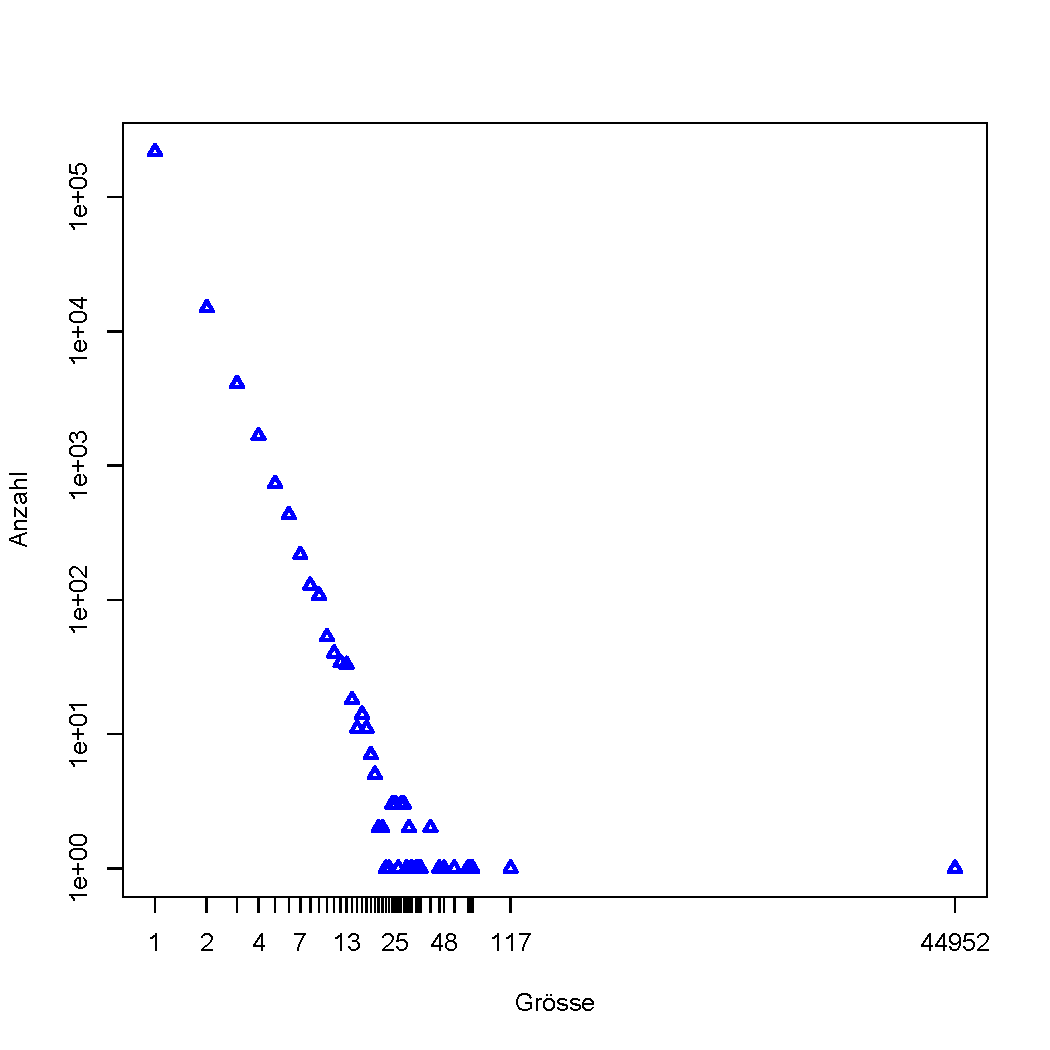
\includegraphics[scale=0.42]{images/component-size.pdf}
  \caption{Gr\"ossenverteilung der starken Zusammenhangskomponenten}
  \label{fig:component-size}
\end{figure}

Der so erhaltene Graph wurde zun\"achst in seine 240382 starken
Zusammenhangskomponenten zerlegt. Die Verteilung der
Komponentengr\"ossen in Abbildung \ref{fig:component-size} zeigt dabei
zwei Extreme: Es existiert eine einzelne gigantische Komponente mit
ca. 45000 Knoten. Demgegen\"uber steht eine geringe Anzahl von kleinen
Komponenten bis zur Gr\"osse 3 , insbesondere aber \"uber 100000
einelementige Komponenten, also einzelne Knoten, die nur
\emph{entweder} ein- oder ausgehende Kanten haben, und \"uber 10000
zweielementige Komponenten, also durch zwei Kanten verbundene
Knotenpaare. Ein erheblicher Anteil der \"uberhaupt vernetzten Knoten
ist also wiederum nur sehr wenig vernetzt.

\begin{figure}[th!]
  \centering
  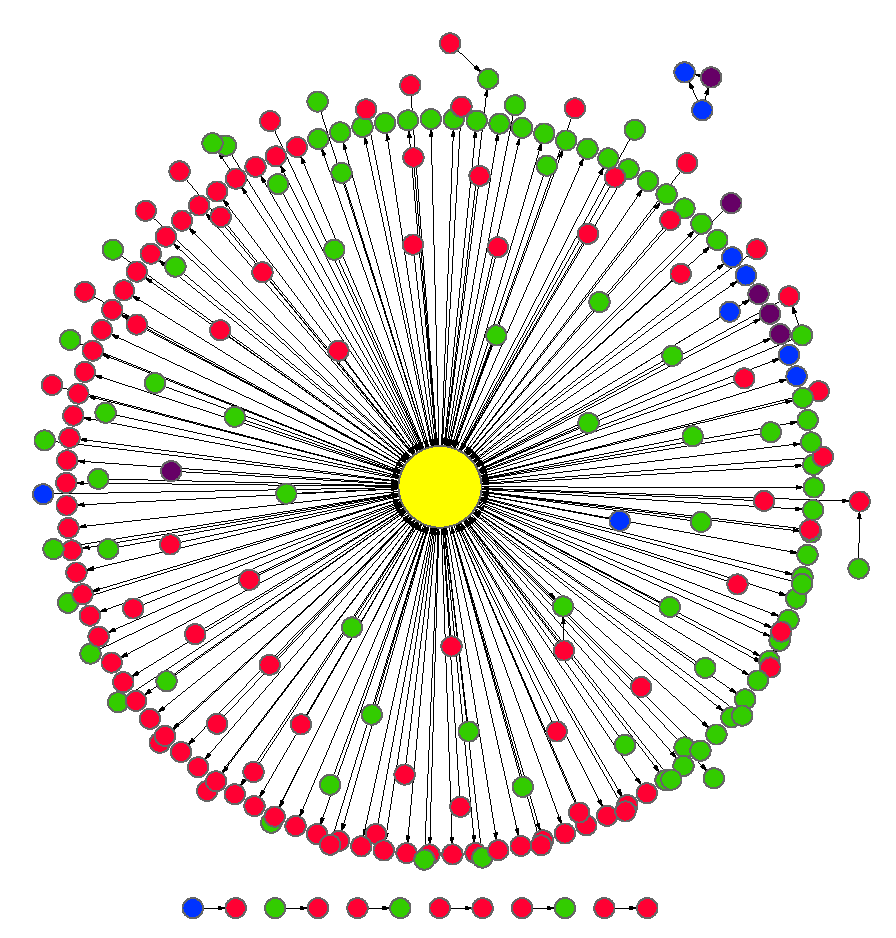
\includegraphics[scale=0.7]{images/component-metagraph-8.pdf}
  \caption{Struktur der starken Zusammenhangskomponenten bis zur
    Grösse 6 (rot = Grösse 6-10, grün = Grösse 11-20, blau = Grösse
    21-30, violett = Grösse $>= 31$, gelb = MSCC)}
  \label{fig:komponenten-struktur}
\end{figure}

Abbildung \ref{fig:komponenten-struktur} zeigt die Struktur der
Zusammenhangskomponenten bis zur Gr\"osse 6, die mit anderen
Komponenten verbunden sind. Es ergibt sich eine sternf\"ormige
Struktur, bei der die kleineren Komponenten fast ausschliesslich mit
der gr\"ossten Komponente verbunden sind und es so gut wie keine
weitere Vernetzung gibt. Um zwei starke Zusammenhangskomponenten
verschmelzen zu lassen, ist nur genau eine Kante in jede Richtung
n\"otig. Es kann also davon ausgegangen werden, dass die Komponenten
nur durch einzelne Kanten, die eben nur in eine Richtung verlaufen
k\"onnen, verbunden sind. Daraus ergibt sich, dass die Mitglieder
der kleinen Komponenten nur eine sehr geringe Signaturaktivit\"at
aufweisen k\"onnen, da andernfalls die Wahrscheinlichkeit f\"ur das Verschmelzen
von Komponenten hoch w\"are und die Anzahl sehr kleiner Komponenten
geringer sein m\"usste.

Die \emph{N\"utzlichkeit} des Web of Trust f\"ur die Teilnehmer, deren
Schl\"ussel nicht in der gr\"ossten starken Zusammenhangskomponente
enthalten sind, ist gering: Die Menge der Schl\"ussel, die von einem
Teilnehmer anhand von Signaturketten verifiziert werden kann,
beschr\"ankt sich zun\"achst auf die eigene Komponente und ist damit
sehr klein. Zwar gibt es auch -- wie oben gezeigt -- Vernetzung
zwischen kleineren Komponenten und der gr\"ossten Komponente. Es
existieren ca. 18000 Knoten, die Knoten aus der gr\"ossten Komponente
direkt \"uber eine einzige Kante errreichen k\"onnen. Allerdings muss
hier beachtet werden, dass das in PGP/GnuPG verwendete
Verifizierungsmodell die L\"ange der verwendbaren Signaturketten
begrenzt -- in der Standardeinstellung von GnuPG auf die maximale
L\"ange 5 (siehe Abschnitt
\ref{sec:das-gnupg-vertrauensmodell}). Schon innerhalb der gr\"ossten
Komponente sind viele k\"urzeste Pfade l\"anger als dieses Maximum
(siehe Abschnitt \ref{sec:kennz-des-graph}). Durch den zus\"atzlichen
Schritt zu einem Knoten innerhalb der gr\"ossten Komponente
verl\"angert sich der Pfad. Insbesondere wenn es sich bei diesen
Knoten um schwach vernetzte Knoten handelt, die am ``Rand'' der
gr\"ossten Komponente liegen, ist die Menge der auf Pfaden benutzbarer
L\"ange erreichbaren Knoten beschr\"ankt. Kann die gr\"osste
Komponente nur indirekt \"uber andere Knoten erreicht werden,
reduziert sich diese Menge noch weiter. Gleiches gilt auch f\"ur die
Erreichbarkeit der Menge von ca. 92000 Knoten, zu denen eine Kante von
Knoten der gr\"ossten Komponente aus besteht. Beachtet werden muss
allerdings die Existenz von zentralen Certificate Authorities im
eigentlich dezentralen Web of Trust. Mit den drei seit 1997 im Rahmen der
``Krypto-Kampagne'' der Zeitschrift c't (siehe Abschnitt
\ref{sec:sozi-komp-des}) verwendeten Zertifizierungsschl\"usseln
wurden insgesamt 23813 derzeit g\"ultige Schl\"ussel
unterschrieben. Von diesen liegen nur 2578 Schl\"ussel innerhalb der
gr\"ossten Komponente. Wenn also nur dem verwendeten
Zertifizierungsprozess und damit diesen drei
Zertifizierungsschl\"usseln vertraut wird, sind immerhin etwa 20000
Schl\"ussel aussserhalb der gr\"ossten Komponente verifizierbar. Es
zeigt sich hier auch die Flexibilit\"at des Web of Trust-Konzeptes,
dass die Integration von zentralen Komponenten in das eigentlich
dezentrale Netz erlaubt.

Insgesamt lassen diese Daten den Schluss zu, dass ausschliesslich die
gr\"osste starke Zusammenhangskomponente Schl\"ussel von Personen
enth\"alt, die sich durch regelm\"assige Signaturaktivit\"aten am Web
of Trust beteiligen und es zur Verifizierung von Schl\"usseln
benutzen. Eine weitergehende Analyse der in den kleineren
Zusammenhangskomponenten enthaltenen Schl\"ussel wird in Abschnitt
\ref{sec:zusammenhangskomponenten-inhaltlich} vorgenommen.

\subsection{Netzwerkstatistiken der gr\"ossten starken
  Zusammenhangskomponente}
\label{sec:kennz-des-graph}

Der induzierte Teilgraph der gr\"ossten starken
Zusammenhangskomponente besteht aus 44952 Knoten und 442960
gerichteten Kanten.

\begin{figure}[th!]
  \centering
  \subfloat[]{\label{fig:indeg-dist} 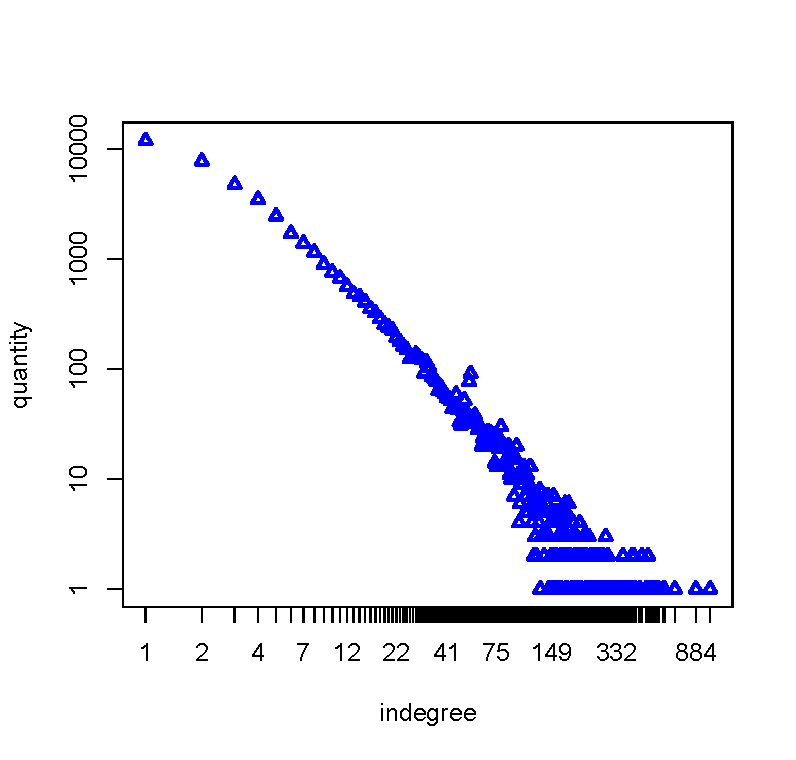
\includegraphics[scale=0.42]{images/indegree-dist.pdf}}
  \subfloat[]{\label{fig:outdeg-dist} 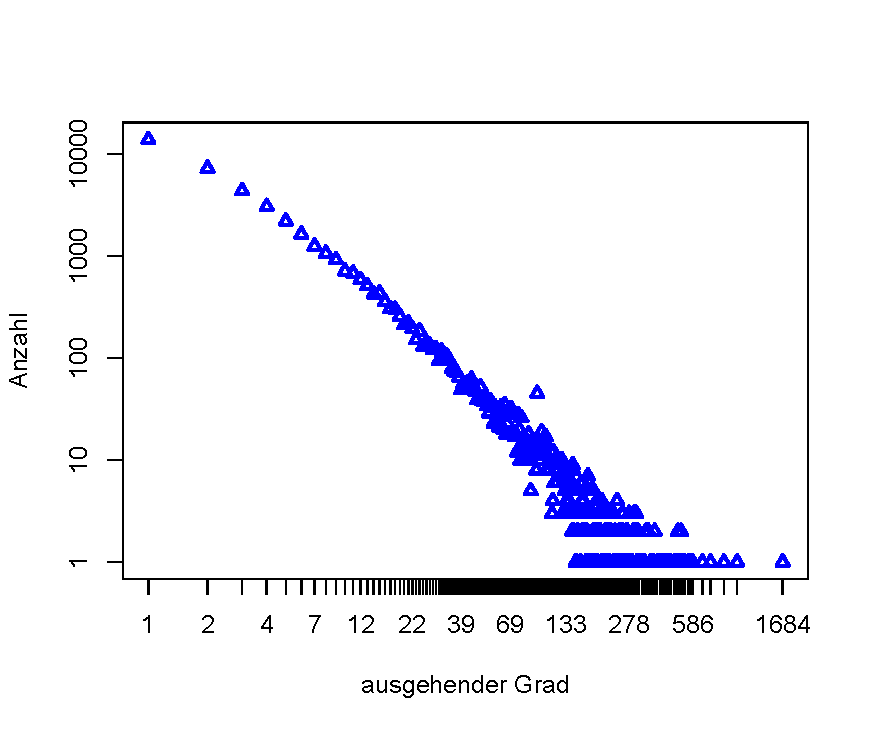
\includegraphics[scale=0.42]{images/outdegree-dist.pdf}}
  \caption{Verteilung der eingehenden \subref{fig:indeg-dist} und
    ausgehenden \subref{fig:outdeg-dist} Knotengrade in der gr\"ossten
    starken Zusammenhangskomponente}
  \label{fig:comsizedist}
\end{figure}

(Kein reines powerlaw).

Unabh\"angig von der konkreten Verteilung kann aber festgehalten
werden, dass es eine (kleine) Anzahl von Knoten mit sehr hohem Grad
gibt. (weiter ausf\"uhren, was das f\"ur das Netzwerk bedeutet -- Hubs
usw.) Orientieren an (Newman -- Email, Bele -- Email). Spekulieren, ob
das mit the rich get richer zu tun hat -- verbinden mit Modell aus
Capkun-Paper.

Es gibt viele Knoten mit geringem Grad, vor allem mit Grad 1. F\"ur
diese Knoten gilt, dass sie nur eine M\"oglichkeit haben, um
Signaturketten zu bauen. Warum ist das schlecht? Weil diese Knoten
zumindest f\"ur die ersten Schritte in der Signaturkette keine
Redundanz haben. Wenn sie dem ersten Knoten nicht vertrauen, kommen
sie nirgendwohin. F\"ur die Knoten mit indegree=1 gilt andersherum,
dass keine redundanten Signaturketten dorthin m\"oglich sind. Dem
einzigen Knoten, der sie ihn signiert hat, muss vertraut werden, oder
der Schl\"ussel kann \"uberhaupt nicht verifiziert werden. Ausserdem
gilt f\"ur diese Knoten, dass das Expiren eines einzigen Knoten (wie
viele Knoten mit expiredate gibt es?) sie komplett vom Netz abtrennen
w\"urde.

\begin{figure}[th!]
  \centering
  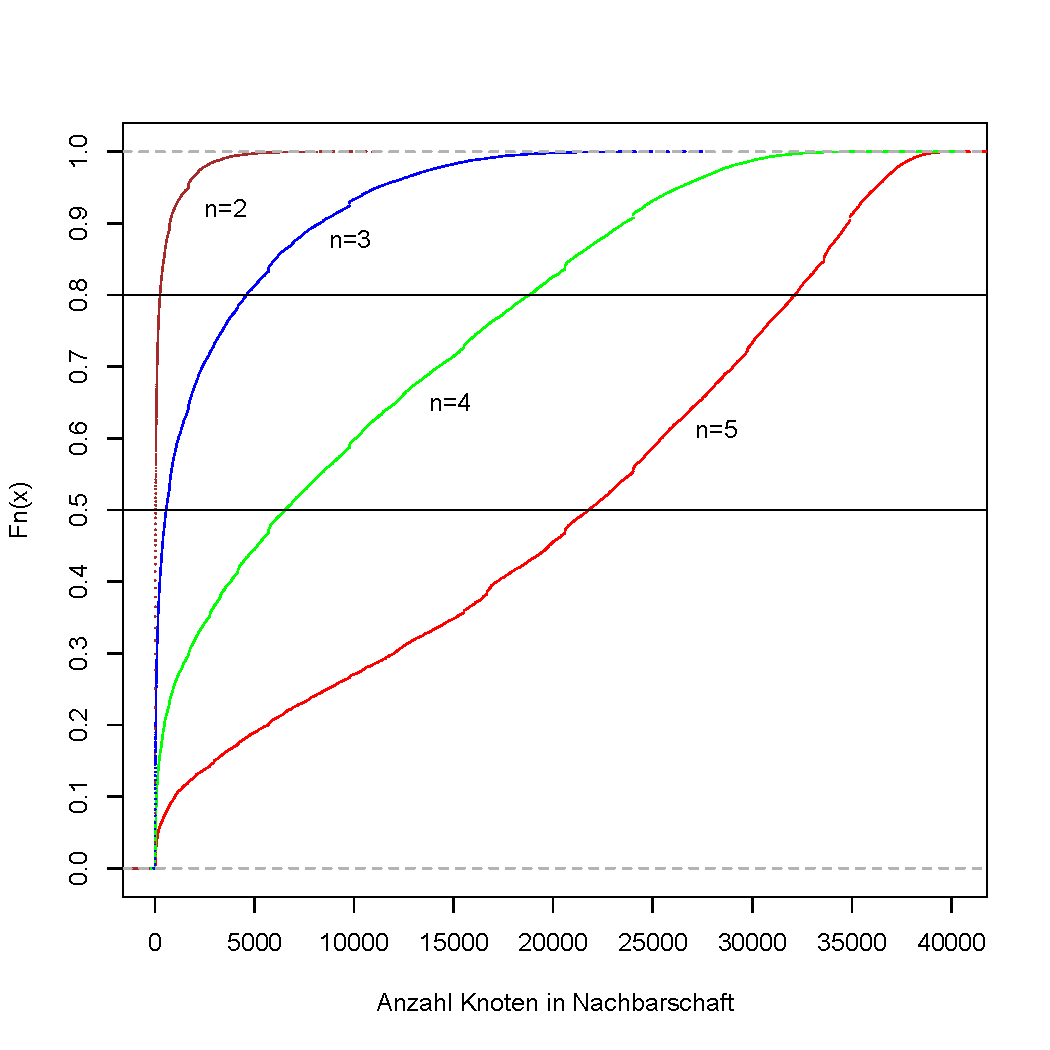
\includegraphics[scale=0.6]{images/neighbourhood-cdf.pdf}
  \caption{Kumulative Verteilungsfunktion der Nachbarschaften}
  \label{fig:neighbourhood-cdf}
\end{figure}

Hier geht es um die Frage, wie \emph{n\"utzlich} das Netzwerk f\"ur
seinen Zweck, n\"amlich die Verifizierung von Schl\"usseln durch
Signaturketten, eigentlich ist.

\begin{figure}[th!]
  \centering
  \subfloat[]{\label{fig:avg-pathlen}\includegraphics[scale=0.3]{images/pathlen-dist.pdf}}
  \subfloat[]{\label{fig:eccentricity}\includegraphics[scale=0.3]{images/ecc-dist.pdf}}
  \caption{Verteilung der durschnittlichen Pfadl\"angen
    \subref{fig:avg-pathlen} und der Eccentricity
    \subref{fig:eccentricity} in der gr\"ossten starken Zusammenhangskomponente}
  \label{fig:pathlen-dist}
\end{figure}


\subsection{Betweeness Centrality}
\label{sec:betw-centr}

\subsection{Struktur der starken Zusammenhangskomponenten}
\label{sec:struktur-der-starken}



\section{Eigenschaften einzelner Schl\"ussel, zeitliche Entwicklung}
\label{sec:result-key-properties}

\cite{Stevens2009}

\begin{figure}[th!]
  \centering
  \subfloat[]{\label{fig:size-dev-whole} \includegraphics[scale=0.3]{images/whole-size-time.pdf}}
  \subfloat[]{\label{fig:size-dev-mscc} \includegraphics[scale=0.3]{images/mscc-size-time.pdf}}
  \caption{Zeitliche Entwicklung der Gr\"osse des gesamten
    Schl\"usselbestandes \subref{fig:size-dev-whole} und der
      gr\"ossten starken Zusammenhangskomponente \subref{fig:size-dev-mscc}}
  \label{fig:size-dev}
\end{figure}


\begin{figure}[th!]
  \centering
  \subfloat[]{\label{fig:pkalg-whole} 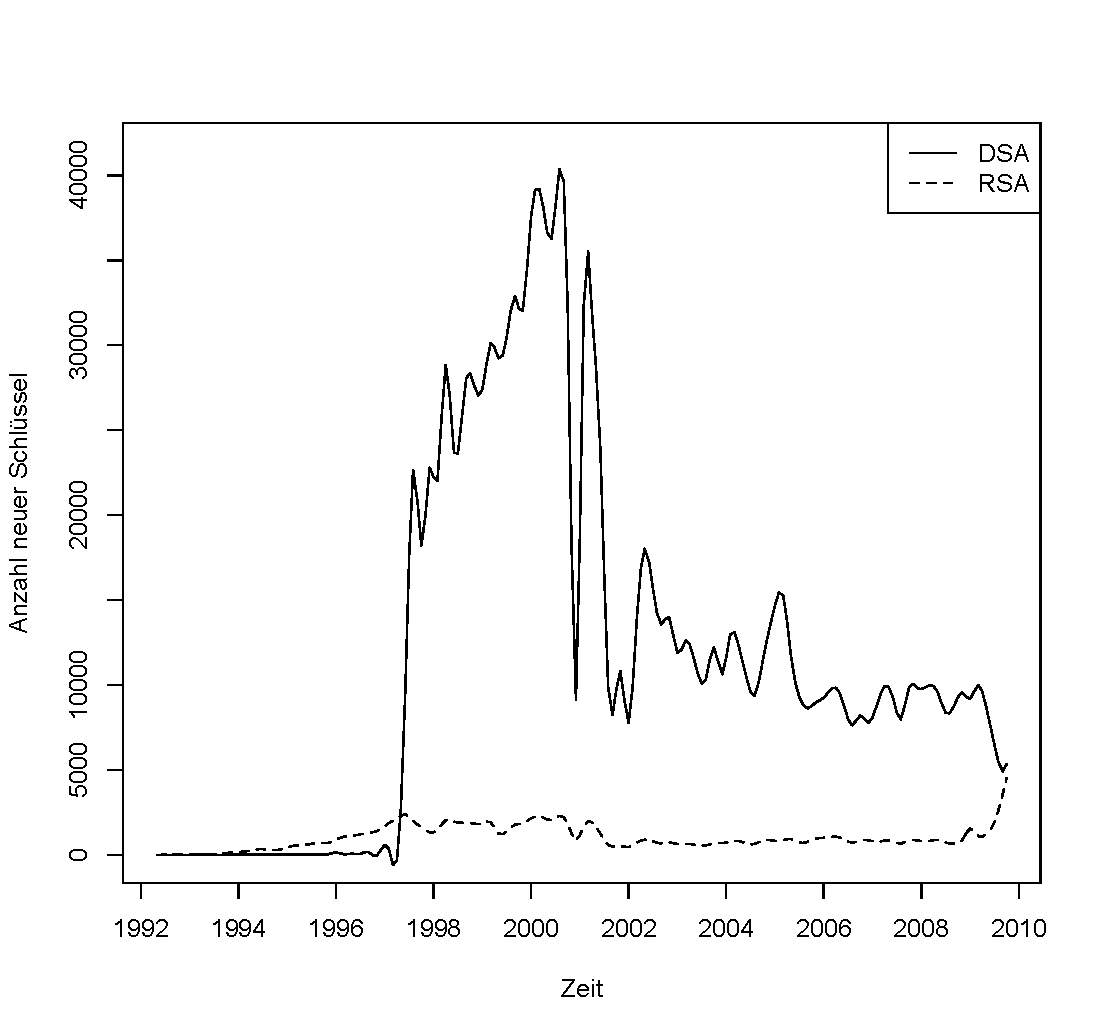
\includegraphics[scale=0.4]{images/whole-pkalg-use.pdf}}
  \subfloat[]{\label{fig:pkalg-mscc} 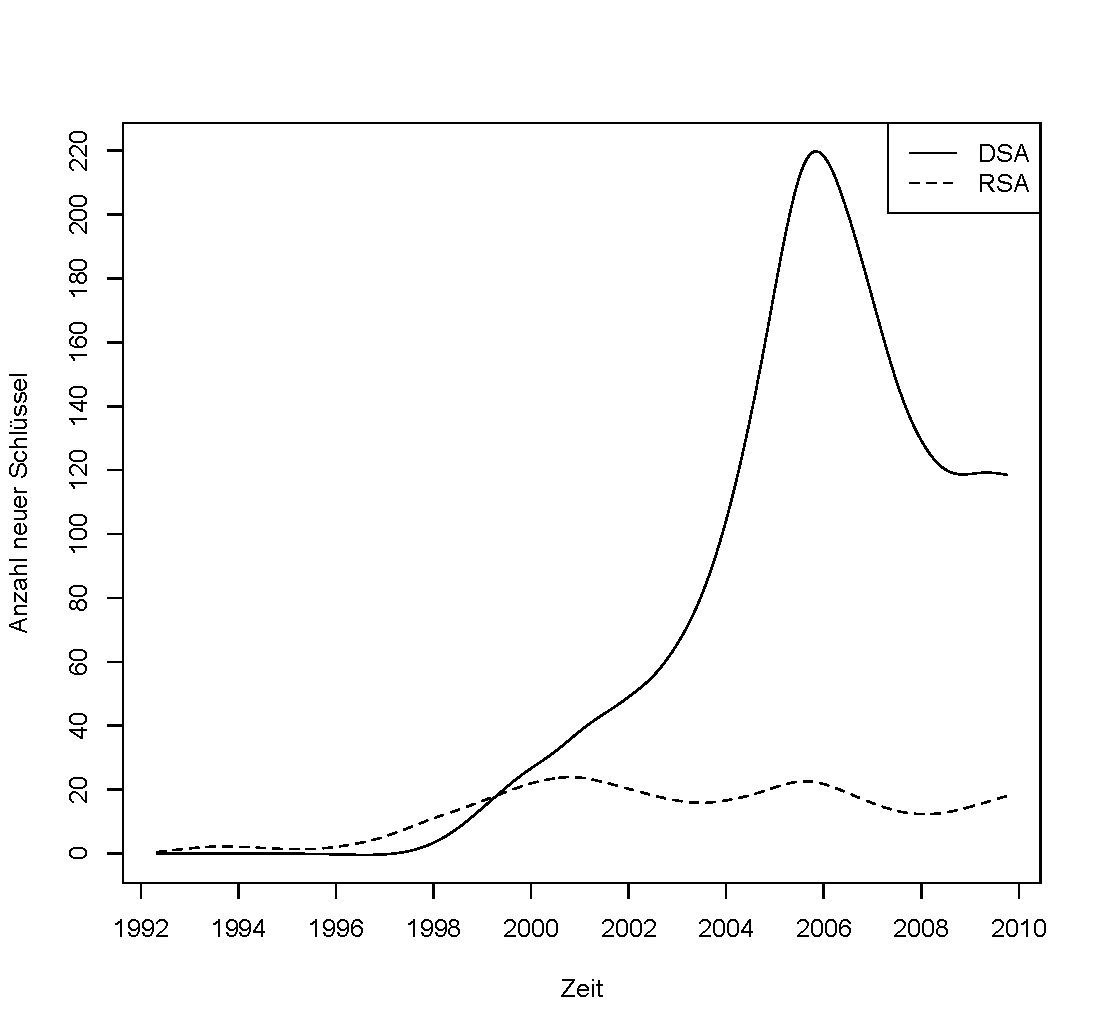
\includegraphics[scale=0.4]{images/mscc-pkalg-use.pdf}}
  \caption{Zeitliche Entwicklung der Gr\"osse des gesamten
    Schl\"usselbestandes \subref{fig:size-dev-whole} und der
      gr\"ossten starken Zusammenhangskomponente \subref{fig:size-dev-mscc}}
  \label{fig:size-dev}
\end{figure}

\section{Zusammenhangskomponenten und Communities}
\label{sec:result-zusamm-und-comm}

\subsection{Communities}
\label{sec:result-communities}

Die Zerlegung des gerichteten Graphen mit dem Algorithmus von Rosval
et al. lieferte keine verwertbaren Ergebnisse. Zwar wurde eine
Zerlegung in 2869 Partitionen berechnet. Allerdings gilt f\"ur die
grosse Mehrzahl dieser Knotenmengen, dass der durch sie induzierte
Teilgraph \"uberhaupt keine Kanten hat. Nur f\"ur ca. 160 Partitionen
hat der jeweils induzierte Teilgraph Kanten, in allen F\"allen
allerdings sehr wenige (zwischen 1 und 104 f\"ur eine Partition der
Gr\"osse 682). Dass die Knoten einer Partition in allen F\"allen so
gut wie keine interne Vernetzung haben und damit der Definition von
Communities absolut nicht entsprechen, ist ein klarer Hinweis, dass
die berechnete Zerlegung die tats\"achliche modulare Struktur des
Graphen nicht sinnvoll wiedergibt. Dass der Graph in der Tat eine
ausgepr\"agte modulare Struktur hat, zeigen die anhand des
ungerichteten Graphen berechneten Zerlegungen, die auch unter
inhaltlichen Gesichtspunkten Sinn ergeben. Diese Struktur kann sich
auch nicht erst durch die Reduzierung des gerichteten auf einen
ungerichteten Graphen ergeben. Die berechnete Zerlegung mit etlichen
grossen Partitionen ohne interne Vernetzung ist in keinem Fall ein
sinnvolles Ergebnis eines Community-Algorithmus und spricht daher
f\"ur eine fehlerhafte Berechnung. Ob diese allerdings auf Fehler in
der verwendeten Implementierung der Autoren
\footnote{http://www.tp.umu.se/~rosvall/code.html} oder auf Fehler im
Algorithmus zur\"uckgeht, ist nicht bekannt.

F\"ur die restlichen Methoden wurde der Graph auf einen ungerichteten
Graphen reduziert. Dazu wurde jede einzelne gerichtete Kante in eine
ungerichte Kante umgewandelt. Aus dem gerichteten Graphen mit 446326
Kanten ergab sich so ein ungerichteter Graph mit 295425 Kanten.

F\"ur die COPRA-Berechnung wurden -- wie in \cite{Gregory2010}
vorgeschlagen -- Berechnungen mit unterschiedlichen Werten $v$
durchgef\"uhrt, um den ``besten'' Wert im Sinne der Modularity zu
ermitteln. Dabei ergaben sich mit steigender maximaler \"Uberlappung
$v$ nur bis $v\le 3$ steigende Modularity-Werte, dar\"uber hinaus
fielen sie kontinuierlich ab. Deshalb wurde die Berechnung mit $v=3$
verwendet. Die dort berechneten Modularity-Werte hatten eine geringe
Standardabweichung von 0,003. Dieses Ergebnis kommt unerwartet. In
\cite{Gregory2010} ergaben sich f\"ur ein PGP-Web-of-Trust-Netzwerk
mit 10680 Knoten bis zu $v=9$ ansteigende Modularity-Werte. Das
(lokale) Maximum bei geringem $v$ f\"ur das hier verwendete Netzwerk
k\"onnte darauf hinweisen, dass seine Community-Struktur keine
signifikante \"Uberlappung aufweist. Ein weiterer Hinweis darauf ist,
dass die Einf\"uhrung der \"Uberlappung mit $v=3$ gegen\"uber der
nicht \"uberlappenden Berechnung mit $v=1$ f\"ur die Modularity
(Tabelle \ref{tab:mod-result}) keinen signifikanten Anstieg
brachte. Auch die Zuordnung zu Gruppen bzw. Keysigning-Parties
(Tabelle \ref{tab:assign}) und die Verteilung der Gr\"osse der
Communities (Abbildungen \ref{fig:comsize-copra} und
\ref{fig:comsize-copra1}) \"ahneln sich weitgehend. Alternativ
k\"onnte dieses Ergebnis allerdings auch in einem nicht-optimalen
Verhalten des Algorithmus begr\"undet liegen.

\begin{figure}[th!]
  \centering
  \subfloat[]{\label{fig:comsize-copra1} 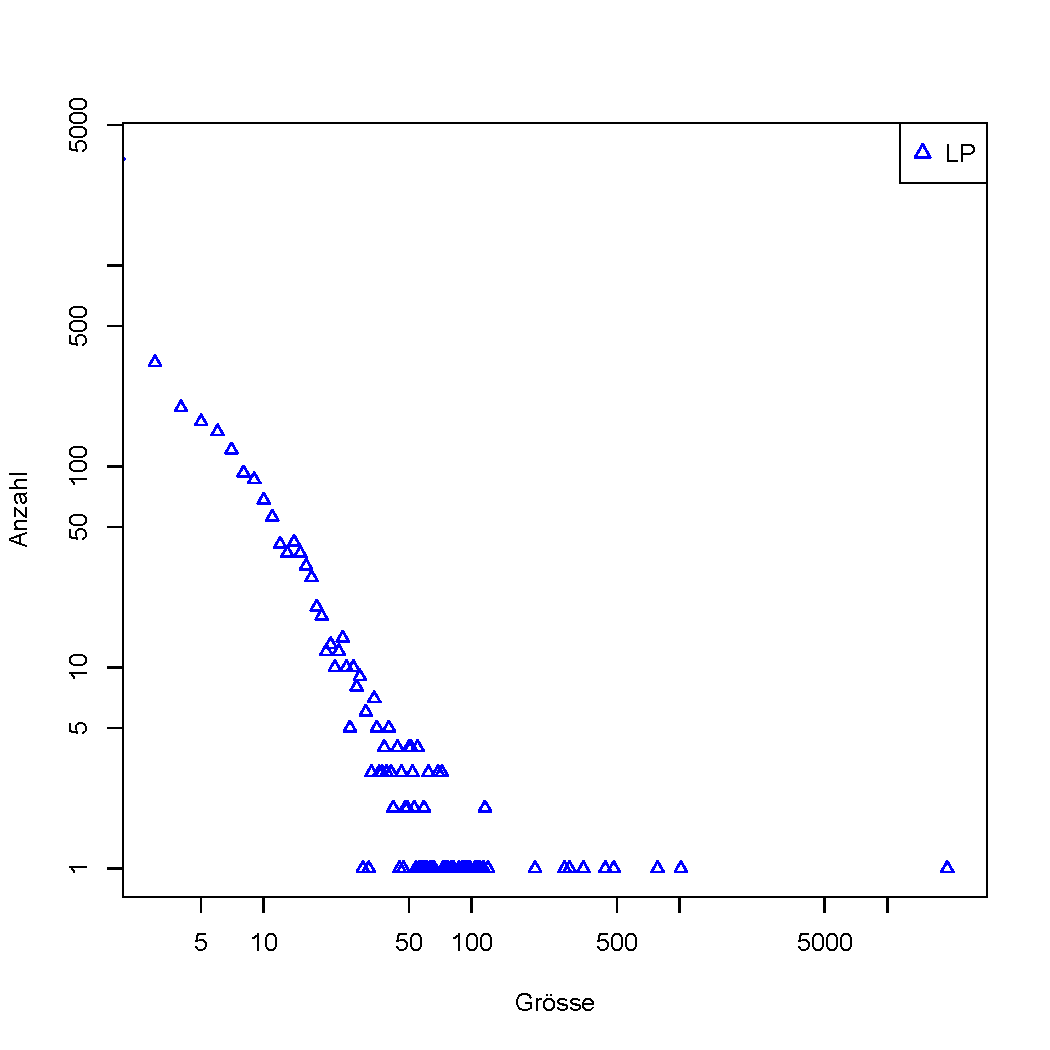
\includegraphics[scale=0.45]{images/community-size-dist_copra1.pdf}}
  \subfloat[]{\label{fig:comsize-copra} 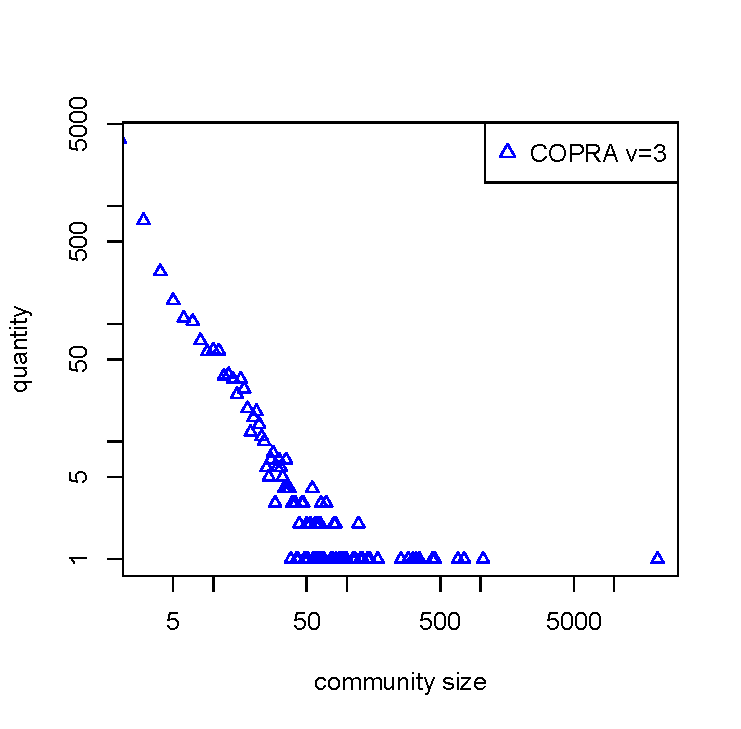
\includegraphics[scale=0.45]{images/community-size-dist_copra.pdf}} \\
  \subfloat[]{\label{fig:comsize-bl2} 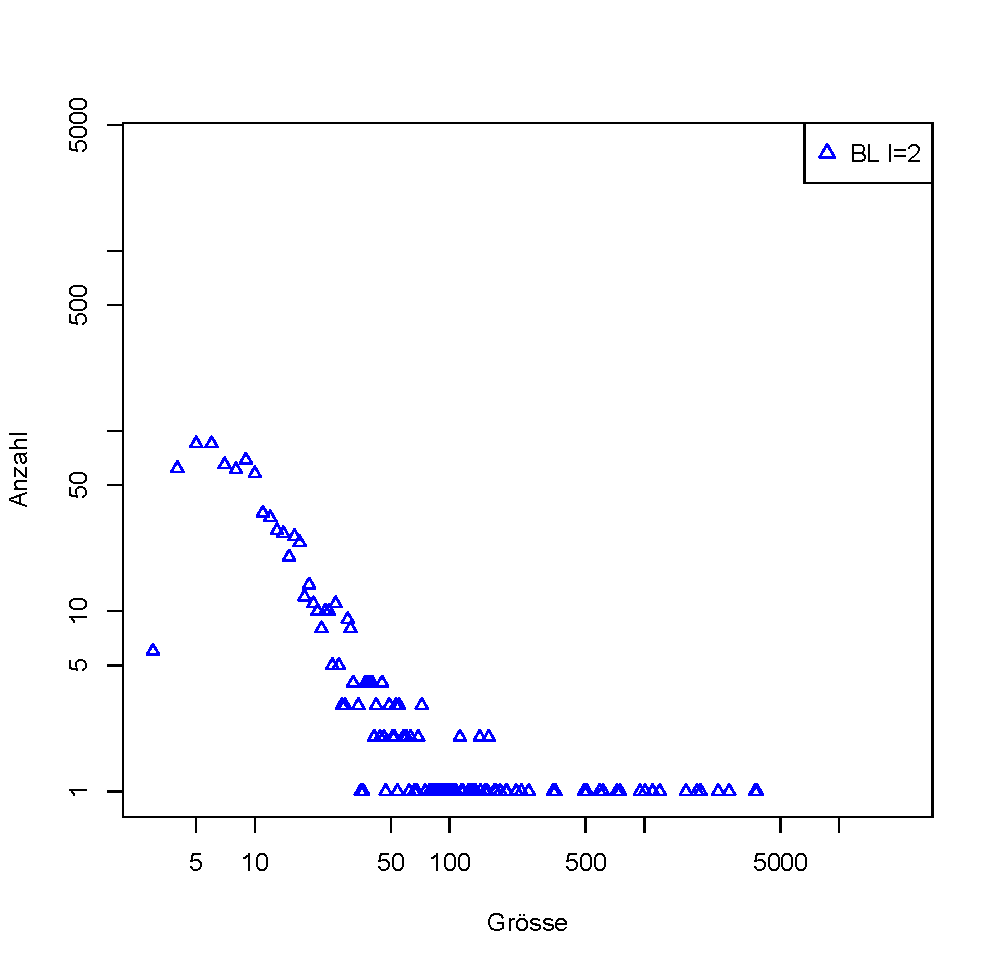
\includegraphics[scale=0.45]{images/community-size-dist_bl2.pdf}} 
  \subfloat[]{\label{fig:comsize-bl5} 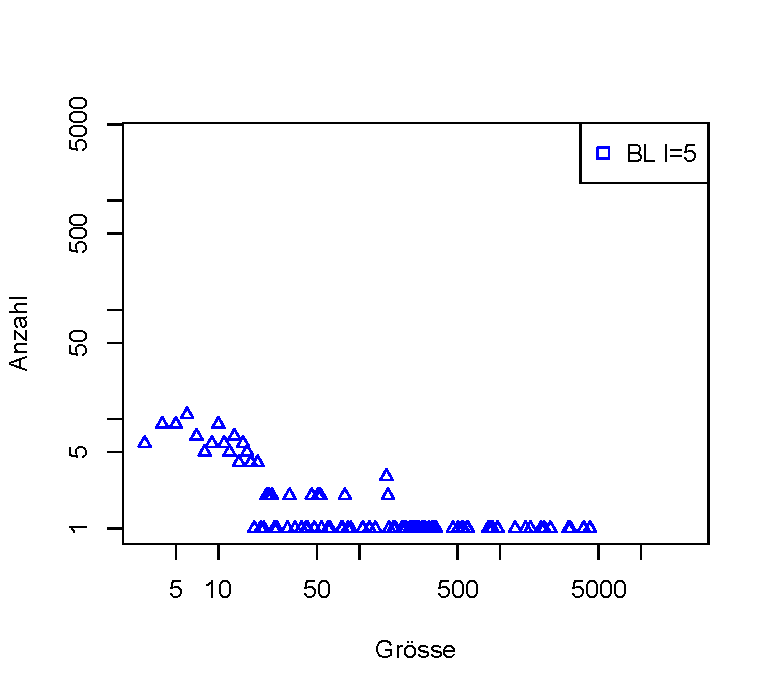
\includegraphics[scale=0.45]{images/community-size-dist_bl5.pdf}} 
  \caption{Gr\"ossenverteilung der Communities}
  \label{fig:comsizedist}
\end{figure}

F\"ur den Algorithmus von Blondel et al. zeigt sich zun\"achst ein
deutlich h\"oherer Modularity-Wert als f\"ur Fastmod. Dieses Ergebnis
gibt also die reine Struktur des Graphen deutlich besser wieder.  Wie
in Abschnitt
\ref{ch:Grundlagen:sec:Netzwerkanalyse:subsec:Communities}
beschrieben, verl\"auft der Algorithmus von Blondel et al. iterativ in
Phasen, in denen jeweils zuerst Knoten einer benachbarten Community
zugeordnet werden, wenn sich dadurch ein Modularity-Gewinn erzielen
l\"asst, und dann die Knoten dieser so entstandenen Communities zu
Knoten in einem neuen Netzwerk verschmolzen werden. Hier werden die
Ergebnisse der Phasen $l=2$ und der letzten Phase $l=5$
betrachtet. F\"ur $l=5$ ergab sich die h\"ochste
Modularity. Allerdings sticht hier die sehr kleine Anzahl von
Communities heraus, die wiederum vergleichsweise gross sein
m\"ussen. Gegen\"uber dem Ergebnis der Phase 2 ergibt sich eine
relativ kleine Steigerung der Modularity, die mit einem erheblichen
Verlust an \emph{Aufl\"osung} erkauft wird\footnote{Die Zerlegungen
  der Phasen 3 und 4 unterschieden sich nur geringf\"ugig von der
  Zerlegung der Phase 5}. Aus Abbildung \ref{fig:comsize-bl2} und
\ref{fig:comsize-bl5} geht hervor, dass diese Reduktion der Anzahl im
Wesentlichen auf das Reduzieren sehr kleiner Communities
zur\"uckgeht. Da der Algorithmus von Blondel et al. genauso wie
Fastmod mittels einer (lokalen) Optimierung der Modularity arbeitet,
k\"onnte dieses Ph\"anomen auf das in der Literatur beschriebene
Aufl\"osungslimit der Modularity-Funktion (bspw. \cite{Fortunato2007}
\cite{Good2009}) zur\"uckzuf\"uhren sein. Es scheint fraglich, ob die
in Relation zur Gr\"osse des Graphen sehr geringe Zahl von 186
Communities die Struktur des Graphen (in Bezug auf die inhaltliche
Analyse) ad\"aquat wiedergibt.

\begin{figure}[ht!]
  \centering
  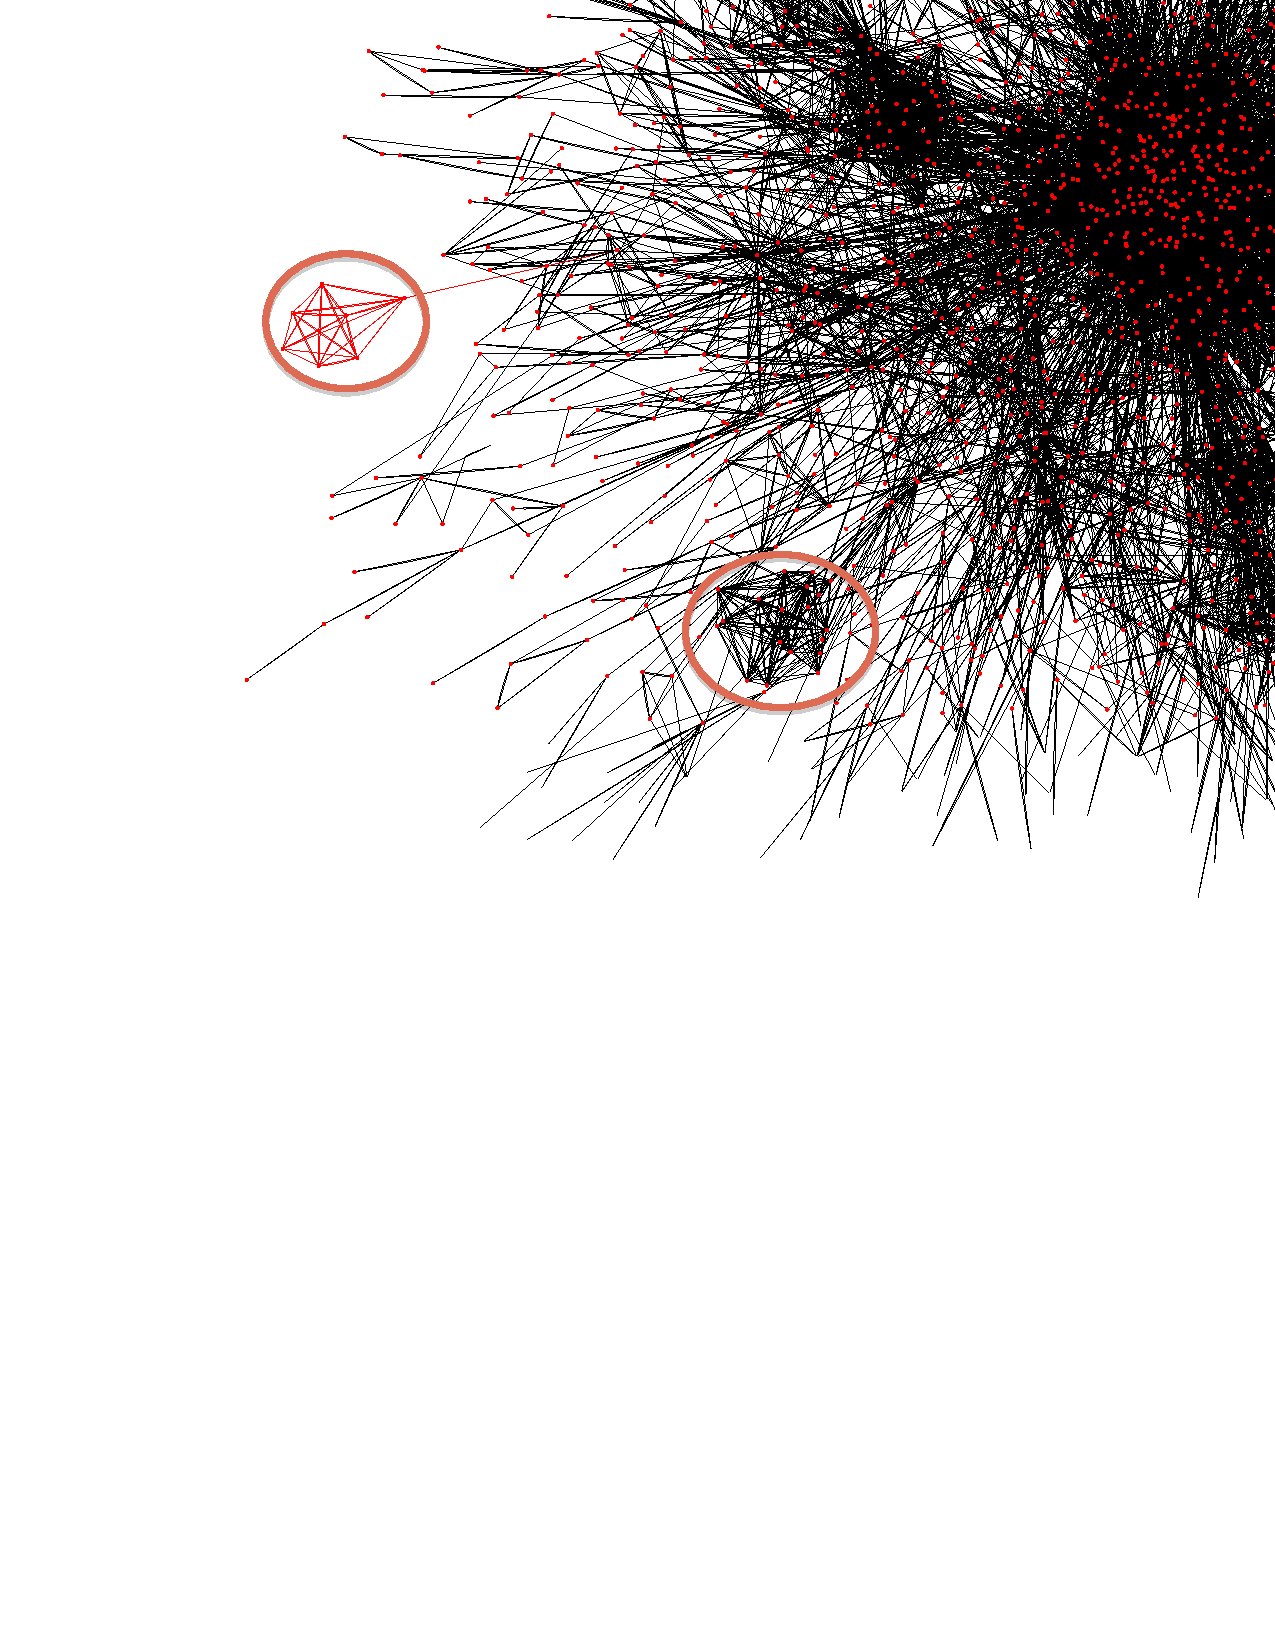
\includegraphics[scale=0.7]{images/blondel-l5-com-c3a5eaab680984b123037897b0be74bf-edit.pdf}
  \caption{Community mit modularen Untereinheiten (Gr\"osse 2271,
    Blondel ($l=5$), Force-directed Layout)}
  \label{fig:large-modular}
\end{figure}

Abbildung \ref{fig:large-modular} illustriert dies anhand einer
Community aus der Zerlegung des Algorithmus von Blondel et al. mit
$l=5$, die klar abgegrenzte Untereinheiten enth\"alt, die intuitiv
wieder eigenst\"andige Communities darstellen.

\begin{figure}[th!]
  \centering
  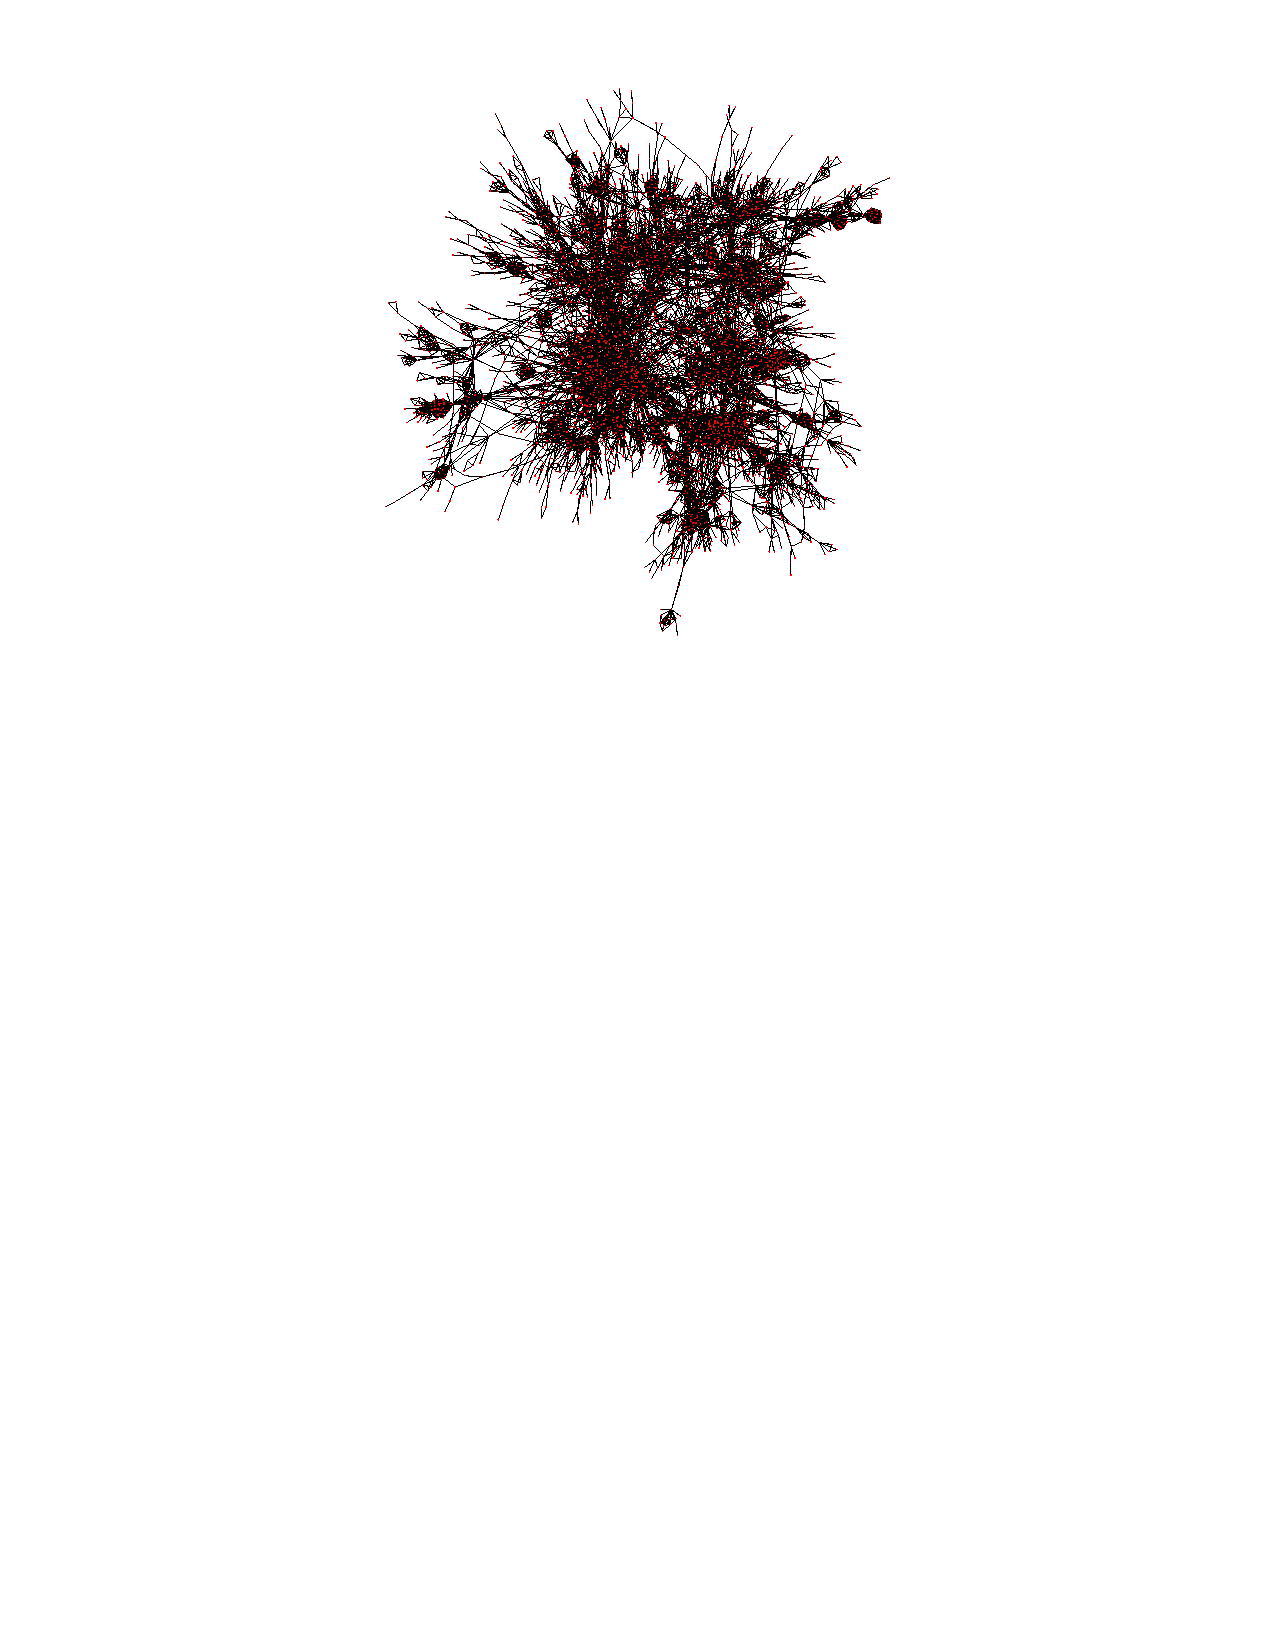
\includegraphics[scale=1.5]{images/fastmod-subgraph-large-modular-6525064ccab580a0b304a3620b197d7a.pdf}
  \caption{Grosse Community mit modularer Struktur (Berechnet mit
    Fast-Modularity, Force-directed layout)}
  \label{fig:large-community-modular}
\end{figure}

Abbildung \ref{fig:large-community-modular} illustriert die begrenzte
Qualit\"at der Fast-Modularity-Zerlegung, die sich im vergleichweise
niedrigen Modularity-Wert niederschl\"agt. In der Zeichnung des
induzierten Teilgraphen einer grossen Community sind etliche dicht
gezeichnete Zusammenballungen von Knoten zu sehen, die nur wenige
Kanten nach aussen haben. Diese k\"onnen als Community-artige
Strukturen interpretiert werden. Zwar kann argumentiert werden, dass
die Zeichnung die Struktur des Teilgraphen nicht notwendigerweise
sinnvoll wiedergibt, dass also die dichten Teilbereiche in der
Zeichnung nur Artefakte der Zeichenmethode darstellen. Allerdings
zeigt Noack, dass starke \"Ubereinstimmungen zwischen einer
energieoptimalen Einbettung eines Graphen in die Ebene nach der
Force-directed-Methode und einer Partitionierung eines Graphen mit
optimaler Modularity bestehen \cite{Noack2009}. Es scheint daher
gerechtfertigt, eine Zeichnung eines Graphen (Force-directed) mit
markanten dichten Bereichen als Indiz f\"ur eine modulare Struktur
dieses Graphen zu betrachten.

\begin{table}[t]
  \centering
  \footnotesize
  \begin{tabular}{l|c|c|c}
    Algorithmus & Modularity & Communities &
    Enthaltene Knoten \\
    \hline
    FM & 0,596 & 552 & 44611 \\
    \hline
    BL ($l=2$)& 0,701 & 936 & 44934 \\
    BL ($l=5$)& 0,710 & 186 & 44934 \\
    \hline
    COPRA ($v=1$) & (0,780) & 1421 & 42205 \\
    COPRA ($v=3$) & (0,786) & 1354 & --- \\

  \end{tabular}
  \caption{Modularity-Werte, Anzahl der Communities mit mehr als 3
    Knoten sowie die Anzahl der insgesamt in diesen Communities (>3) enthaltenen
    Knoten 
    f\"ur die Algorithmen Fast-Modularity (FM), Label-Propagation
    (LP), Blondel et al. (BL) auf Level 2 und 5 sowie COPRA. Die
    Modularity-Werte f\"ur COPRA entsprechen der Modularity-Definition
    f\"ur \"uberlappende Zerlegungen nach \cite{Nicosia2009} und k\"onnen mit den anderen
    Werten nicht verglichen werden.}
  \label{tab:mod-result}
\end{table}

Aus Tabelle \ref{tab:mod-result} geht hervor, dass sich -- zumindest
im Fall von Fastmod und Blondel et al. -- fast alle Knoten des Graphen
in einer Community wiederfinden, die mindestens die Gr\"osse 4 hat. In
Abschnitt \ref{sec:result-allg-merkm-des} wurde gezeigt, dass ein
erheblicher Anteil der Knoten einen sehr geringen Grad von 1 oder 2
hat. Da solche Knoten mangels Kanten nicht selbst eine dichte
Vernetzung herstellen k\"onnen, m\"ussen sie Mitglied in Communities
sein, in denen Knoten mit h\"oherem Grad sowohl die interne Vernetzung
der Community als auch die Vernetzung der Community mit anderen
erzeugen. COPRA scheint hingegen dazu tendieren, deutlich mehr Knoten
in Communities sehr kleiner Gr\"osse mit 3 oder weniger
unterzubringen. Dieses Verhalten k\"onnte dazu f\"uhren, dass die
Aussagekraft der Zerlegung in Bezug auf die realen Communities
geschw\"acht wird, wenn viele Knoten auf diese Art abgespalten werden.

Gegen\"uber der COPRA-Zerlegung mit $v=1$ zeigt die Zerlegung mit
$v=3$ eine deutlich gr\"ossere Anzahl von Communities der Gr\"osse 3
und 4. Abgesehen davon \"ahneln sich die Gr\"ossenverteilungen aber
weitgehend. Beide enthalten eine charakteristische sehr grosse
Community mit ca. 19000 bzw. ca. 21000 Mitgliedern. Demgegen\"uber
bietet die Blondel-Zerlegung mit $l=2$ eine deutlich geringere Anzahl
solcher sehr kleiner Communities, daf\"ur aber eine h\"ohrere Zahl
mittlerer (mehr als 100 Mitglieder) und insbesondere eine h\"ohere
Zahl sehr grosser (zwischen 500 und 5000 Mitglieder) Communities.  Die
beiden Algorithmen konvergieren nicht gegen ein gemeinsames Optimum,
sondern liefern Ergebnisse, die sich qualitativ stark unterscheiden.

Der insgesamt recht hohe Modularity-Wert weist darauf hin, dass der
Graph in der Tat eine ausgepr\"agte modulare Struktur hat, wie dies
von einem sozialen Netzwerk erwartet wird.

Die Abbildungen \ref{fig:metagraph-com-copra} und
\ref{fig:metagraph-com-blondel2} zeigen die Struktur der Communities
f\"ur die Zerlegungen COPRA ($v=1$) und Blondel ($l=2$). Auff\"allig
ist hier insbesondere die teilweise sternf\"ormige Struktur der
COPRA-Zerlegung. Ein signifikanter Anteil der kleineren Communities
ist rund um die zentrale Community der Gr\"osse ca. 19000 angeordnet
und im wesentlichen nur mit dieser vernetzt. Diese Struktur weist
gewisse \"Ahnlichkeiten zur Struktur der starken
Zusammenhangskomponenten auf (siehe Abschnitt
\ref{sec:struktur-der-starken}). Diese sind ebenfalls sternf\"ormig um
eine zentrale Komponente angeordnet, die die Gr\"osse der anderen um
mehrere Gr\"ossenordnungen \"ubertrifft. Allerdings sind im Fall der
Community-Struktur noch eine Reihe mittelgrosser Communities
vertreten, die dieses Muster etwas st\"oren. Das sternf\"ormige Muster
der Zusammenhangskomponenten wiederholt sich also in etwa innerhalb
der gr\"ossten Zusammenhangskomponente auf einem anderen Level. Es
k\"onnte daher spekuliert werden, ob das Netzwerk eine
\emph{Selbst\"ahnlichkeit} aufweist, wie sie f\"ur eine Reihe von
komplexen Netzwerken gezeigt wurde\cite{Song2005}. Dieser Frage wurde
allerdings im Rahmen dieser Arbeit nicht weiter nachgegangen. Im
Vergleich dazu zeigt sich in der Struktur der Blondel-Communities die
etwas ausgewogenere Gr\"ossenverteilung. Zwar sind auch hier viele
kleine Communities sternf\"ormig um die zentralen Communities
angeordnet, verteilen sich hier aber auf mehrere solcher grossen
zentralen Communities.

\begin{figure}[h!]
  \centering
  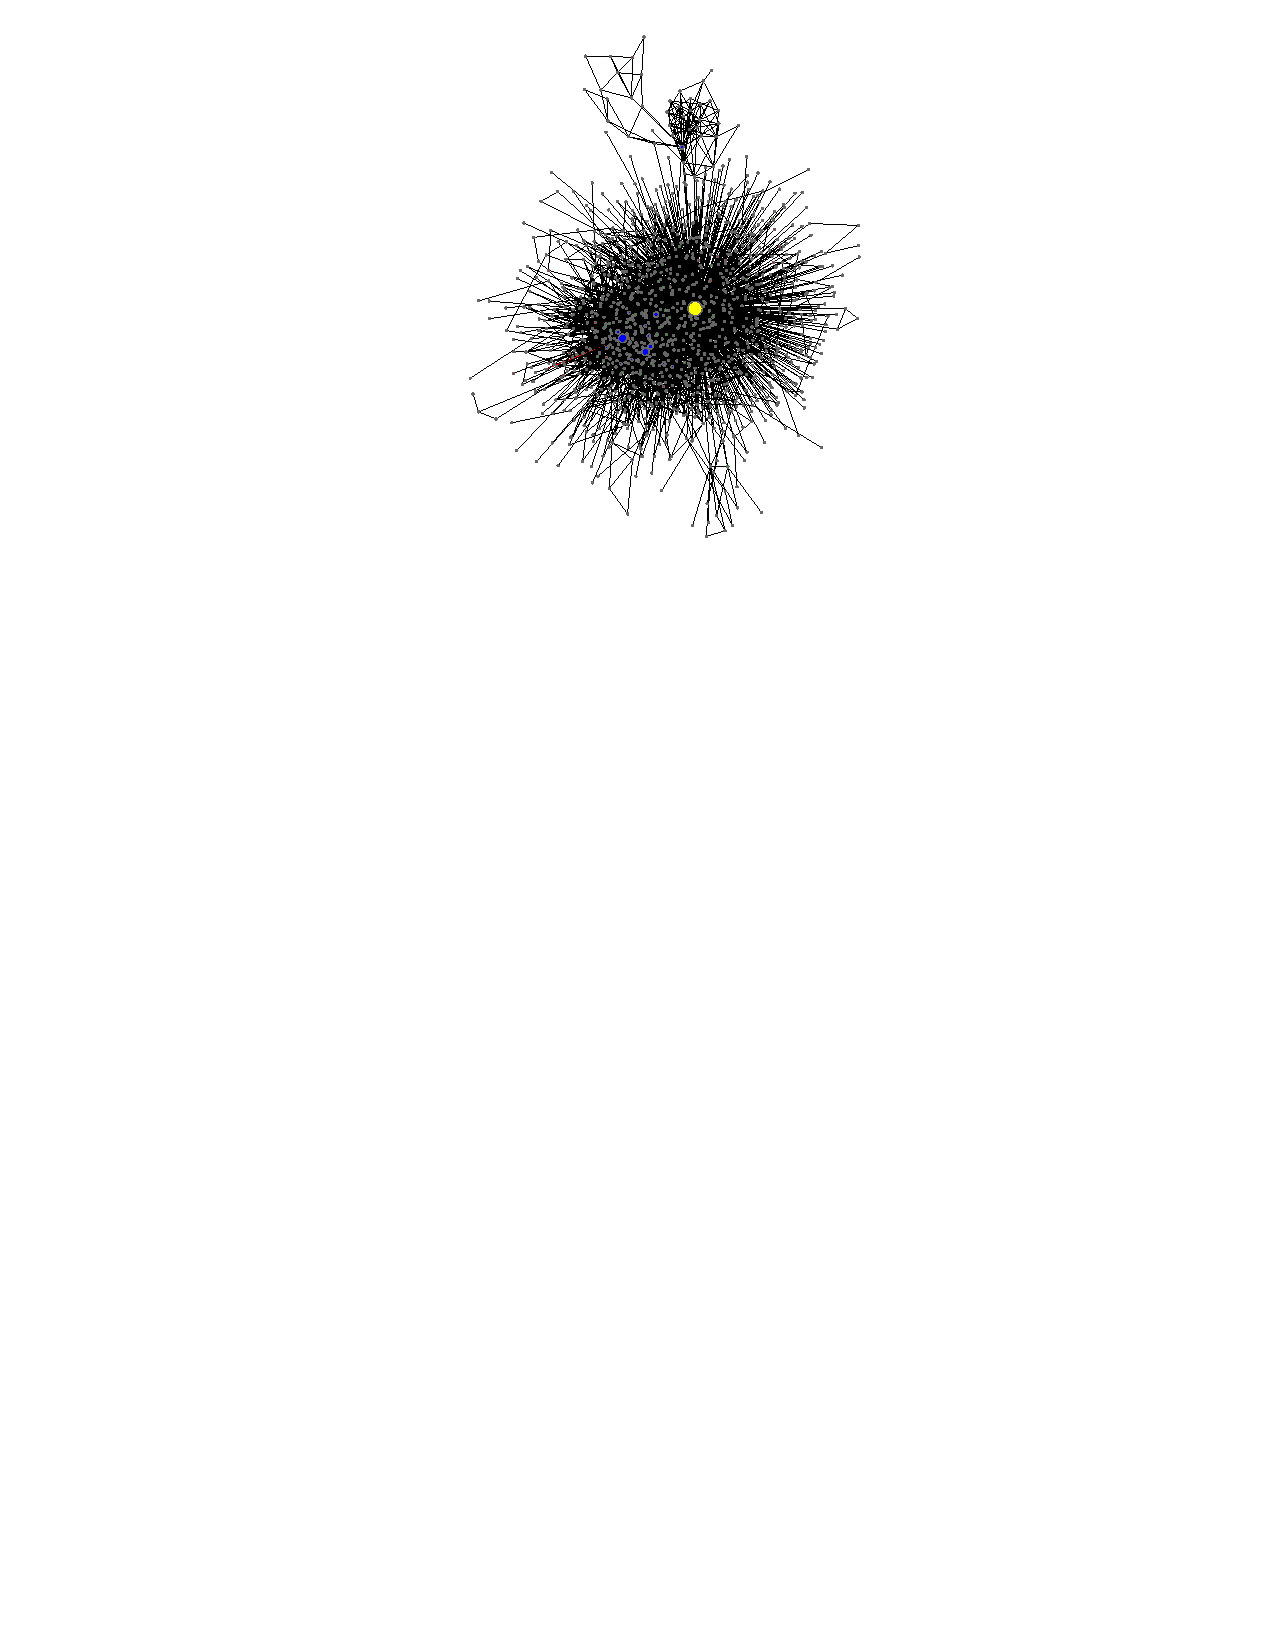
\includegraphics[scale=2]{images/metagraph-copra1-minsize5.pdf}
  \caption{Struktur der Communities (COPRA ($v=1$) (rot: Gr\"osse
    $<10$, gr\"un: Gr\"osse $<100$, blau: Gr\"osse < 1000, gelb:
    Gr\"osse > 1000).}
  \label{fig:metagraph-com-copra}
\end{figure}

\begin{figure}[h!]
  \centering
  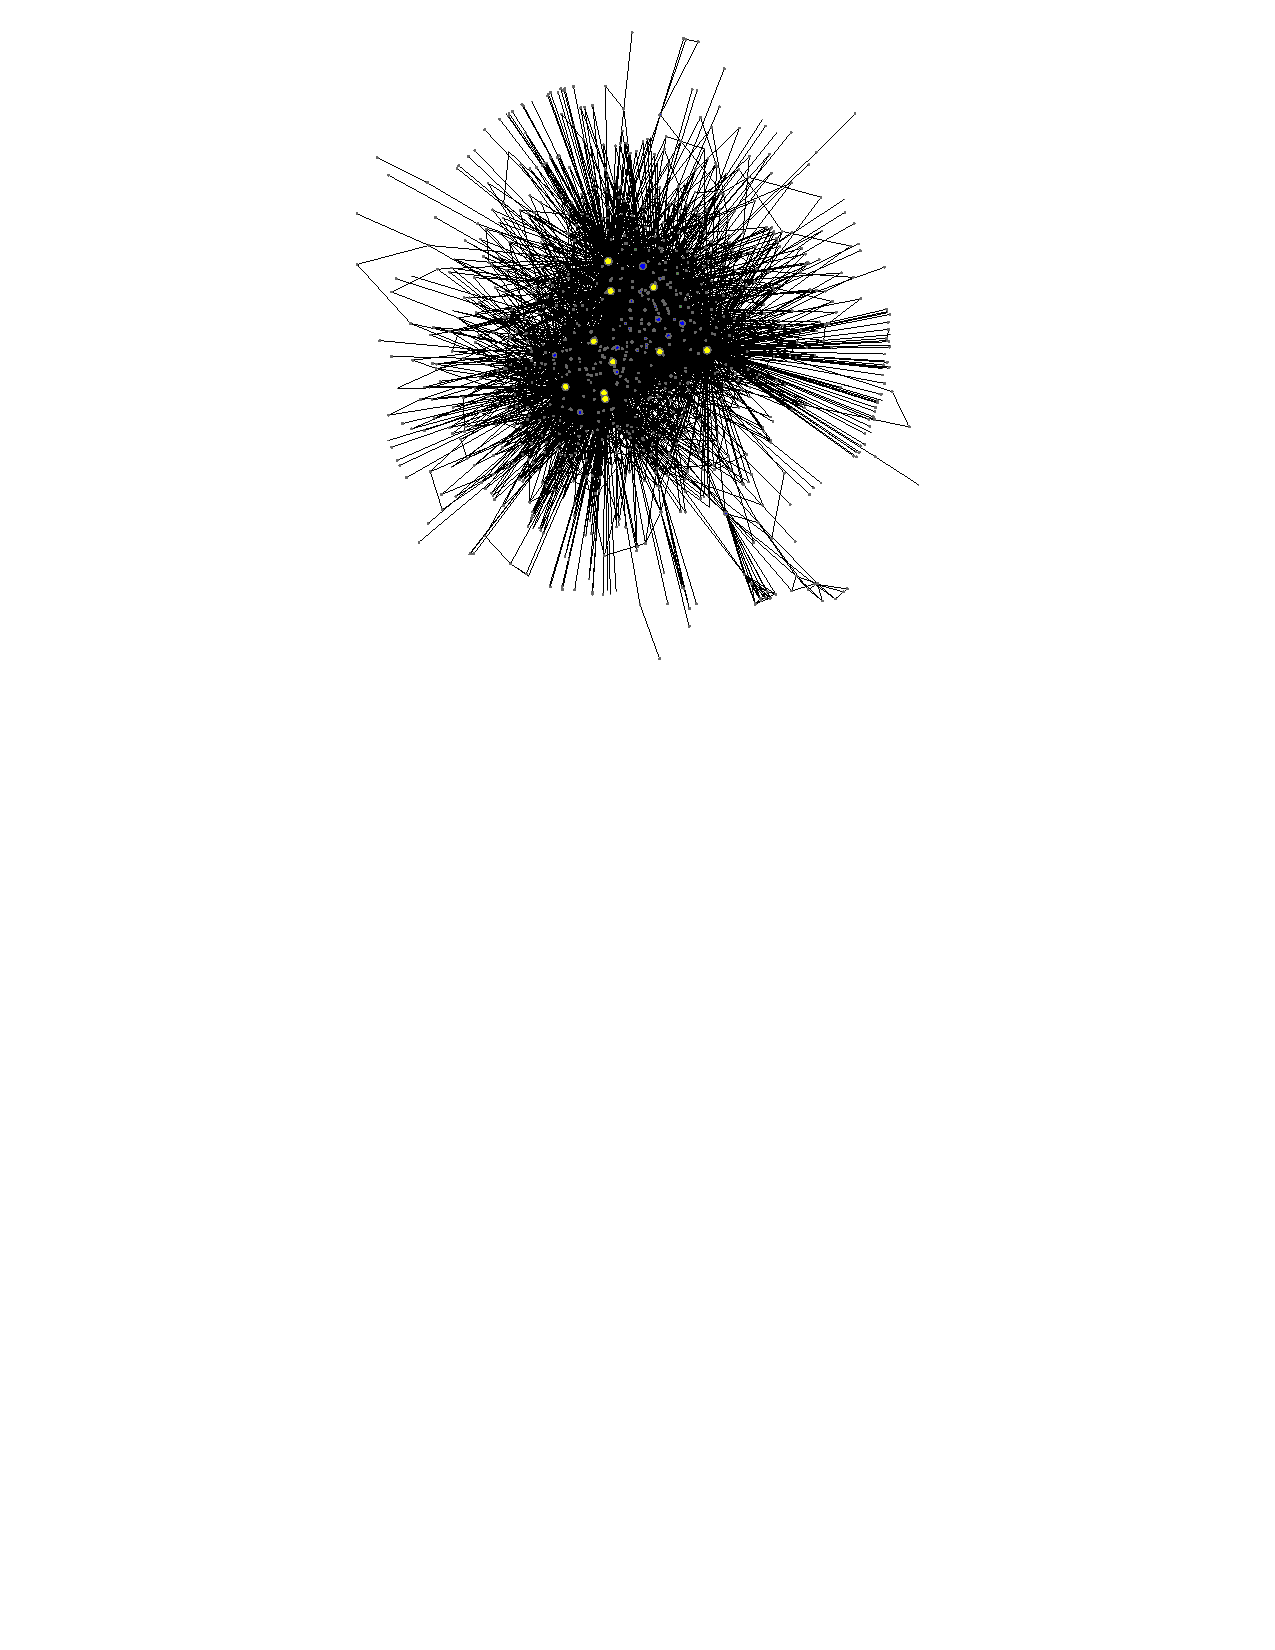
\includegraphics[scale=1.6]{images/metagraph-blondel2-minsize4.pdf}
  \caption{Struktur der Communities (Blondel ($l=5$) (Knotenf\"arbung
    wie in Abb.\ref{fig:metagraph-com-copra})}
  \label{fig:metagraph-com-blondel2}
\end{figure}

\begin{table}[t]
  \centering
  \footnotesize
  \begin{tabular}{l|c|c|c|c|c}
    Algorithmus & TLD-S & TLD-M & SLD-S & SLD-M & SIG \\
    \hline
    FM & 293 (53\%) & 247 (44\%) & 56 (10\%) & 154 (27\%) & 128
    (23\%) \\
    \hline
    BL ($l=2$) & 499 (53\%) & 417 (45\%) & 41 (4\%) & 254 (27\%) & 115 (12\%) \\
    BL ($l=5$) & 85 (47\%) & 85 (47\%) & 15 (8\%) & 38 (21\%) & 26 (14\%) \\
    \hline
    COPRA ($v=1$) & 824 (58\%) & 564 (40\%) & 178 (13\%) & 429 (30\%)
    & 572 (40\%) \\
    COPRA ($v=3$) & 792 (58\%) & 525 (38\%) & 187 (14\%) & 425 (31\%) & 555
    (41\%)
  \end{tabular}
  \caption{SLD-TLD-Zuweisung, TIME-CORR}
  \label{tab:assign}
\end{table}

Aus Tabelle \ref{tab:assign} geht hervor, dass f\"ur alle Zerlegungen
fast alle Communities einer Top-Level-Domain zuordnenbar sind oder von
einer TLD dominiert werden. Werden die generischen Top-Level-Domains
(gTLD: com, org, net, info, ...) abgezogen, verbleiben im Fall von COPRA
noch 519 (38\%) Communities, die einer TLD (und damit einer
\emph{Country-Coded TLD (ccTLD)}) zugeordnet werden k\"onnen und 315
(23\%), die von einer ccTLD dominiert werden. F\"ur die anderen
Zerlegungen ergeben sich \"ahnliche Werte. Damit ist immerhin etwa die
H\"alfte der Communities einem Land zuordnenbar. F\"ur die von einer
gTLD dominierten Communities ergeben Stichproben, dass sich die
Teilnehmer der meisten dieser Communities anhand der Namen zumindest
einem Sprachraum zuweisen lassen.

Dieses Ergebnis ist naheliegend. Wie in Abschnitt
\ref{sec:community-analyse} dargelegt, wird davon ausgegangen, dass
ein wesentlicher Faktor, der das Zustandekommen von Signaturen
beeinflusst, die sozialen Kontakte einer Person sind. Es ist weiterhin
naheliegend, dass sich diese sozialen Kontakte unter anderem aufgrund
von Sprachbarrieren und der r\"aumlichen N\"ahe haupts\"achlich im
Rahmen eines Landes ergeben. Beispielsweise ist f\"ur eine aus
Finnland stammende Person anzunehmen, dass die Mehrzahl ihrer Freunde,
Bekannten, Gesch\"aftspartner und sonstigen Kontakte wieder Finnen
sind.

Zwar k\"onnte argumentiert werden, dass das Internet die geographische
bzw. nationale Beschr\"ankung sozialer Kontakte aufhebt. Allerdings
spielt die geographische N\"ahe eine wichtige Rolle im
Signaturprozess. Die verbreitete Prozedur f\"ur das Signieren eines
Schl\"ussels setzt ein direktes pers\"onliches Treffen der
Signierenden voraus (siehe Abschnitt \ref{sec:sozi-komp-des}). Es ist
anzunehmen, dass die \"uberwiegende Mehrheit der PGP-Benutzer die
meiste Zeit in einem Land und damit in einem geographisch
eingegrenzten Bereich verbleibt. Damit kommen f\"ur diese Mehrheit
\"uberwiegend nur Bewohner des gleichen Landes als Signaturpartner in
Frage. Als Mechanismen f\"ur die internationale Vernetzung kommen dann
etwa internationale Konferenzen in Frage. Nur ein sehr kleiner Teil
der PGP-Benutzer d\"urfte die notwendige internationale Mobilit\"at
aufweisen, so dass sich seine Signaturen nicht \"uberwiegend einem
geographischen Bereich bzw. einem Land zuweisen lassen.

Interessanter f\"ur die Fragestellung ist aber die Erkennung von
Keysigning-Parties und die Zuordnung zu Second-Level-Domains. Im
Vergleich der Algorithmen (Tabelle \ref{tab:assign}) zeigt sich
zun\"achst, dass die COPRA-Zerlegungen bessere Resultate liefern als
die Blondel-Zerlegungen, da hier mehr Communities zugeordnet werden
k\"onnen. Zwar entf\"allt bei COPRA ein grosser Anteil dieser
Zuordnungen auf sehr kleine Communities der Gr\"osse 3 und 4. Die
Aussagekraft solcher kleiner Zuordnungen ist selbstverst\"andlich sehr
begrenzt. Werden diese abgezogen, verbleibt aber immer noch eine
gr\"ossere Zahl zuordnenbarer Communities nichttrivialer Gr\"osse. Aus
den absoluten Zahlen in Tabelle \ref{tab:assign} und den
Gr\"ossenverteilungen in Abbildungen \ref{fig:sld-suredist},
\ref{fig:sld-maybedist} und \ref{fig:time-corrdist} geht hervor, dass
die \"Uberlappung keine wesentlichen Vorteile bringt. Im Vergleich der
Blondel-Zerlegungen zeigt sich, dass das Zusammenpacken von
Communities von Phase $l=2$ zu Phase $l=5$ und der damit verbundene
Aufl\"osungsverlust es erheblich erschwert, die Communities inhaltlich
zuzuordnen. Eine Zerlegung mit h\"oherer Modularity entspricht also im
Allgemeinen nicht einer Zerlegung, die die Struktur realer Communities
besser wiedergibt. Die Zerlegungen des Algorithmus von BLondel et
al. scheinen insgesamt vom Aufl\"osungslimit der
Modularity-Maximierung betroffen zu sein und bieten daher nicht die
notwendige Aufl\"osung, um die Communities besser inhaltlich
analysieren zu k\"nnen.

Insgesamt ist eine tats\"achliche Zuordnung anhand des
80\%-Schwellwerts nur f\"ur sehr wenige Communities von geringer
Gr\"osse m\"oglich. F\"ur den 40\%-Schwellwert und die zeitliche
Korrelation ist die Anzahl zuordnenbarer Communities deutlich
h\"oher. Auch hier entf\"allt allerdings die Mehrzahl auf sehr kleine
Communities.  Dass so gut wie keine Communities mit einer Gr\"osse
\"uber 100 zugeordnet werden k\"onnen, spricht daf\"ur, dass diese
sich nicht anhand dieser einfachen Mechanismen bilden.

Die sehr grosse Community aus der COPRA-Zerlegung k\"onnte vermuten
lassen, dass hier relativ willk\"urlich Knoten zusammengepackt
wurden. Allerdings hat diese Community eine Reihe von Eigenschaften,
die nahelegen, dass diese Gruppierung durchaus Sinn macht. Von 21157
Knoten vef\"ugen 8879 (42\%) \"uber eine E-Mail-Adresse in der
Top-Level-Domain \emph{.de}, w\"ahrend andere -- insbesondere
nicht-deutschsprachige -- ccTLDs deutlich schw\"acher vertreten
sind. Das zeigt einerseits einen \"uberraschend hohen Anteil von
deutschen oder deutschsprachigen Benutzern am Gesamtnetzwerk. Die 8879
Schl\"ussel sind nat\"urlich nur eine Untergrenze, da auch in einer
Vielzahl weiterer Communities deutsche Teilnehmer vorkommen. Ein Grund
f\"ur diese hohe Anzahl deutscher Schl\"ussel k\"onnte in der in
Abschnitt \ref{sec:sozi-komp-des} erw\"ahnten ``Krypto-Kampagne'' der
Zeitschrift c't liegen, die das Bewusstsein f\"ur die Notwendigkeit
der Authentifizierung von Schl\"usseln im deutschsprachigen Raum
deutlich gesteigert haben d\"urfte. Andererseits l\"asst dies den
Schluss zu, dass die enthaltenen Knoten eben nicht willk\"urlich
zusammengepackt wurden, sondern neben ihrer topographischen N\"ahe
auch eine ``inhaltliche'' Gemeinsamkeit aufweisen. Darauf weist auch
hin, dass in dieser Community eine relativ zu anderen SLDs sehr grosse
Anzahl von Schl\"usseln von Mitgliedern des Debian-Projekts enthalten
ist. Diese Community enth\"alt nicht nur knapp die H\"alfte der
Schl\"ussel, sondern mit ca. 260000 Kanten den Grossteil der
\"uberhaupt vorhandenen Kanten. Sie ist also anscheinend intern sehr
dicht vernetzt. Daher scheint es fraglich, ob sie intern wieder eine
schlecht aufgel\"oste modulare Struktur wie in Abbildung
\ref{fig:large-community-modular} hat, die sich in sinnvolle
Untereinheiten zerlegen l\"asst.

\begin{table}
  \centering
  \begin{tabular}{c|c|c}
    Gr\"osse & SLD & Anteil \\
    436 & apache.org & 48\% \\
    130 & nun.org & 82\% \\
    97 & cert.org & 70\% \\
    81 & redhat.org & 68\% \\
    63 & purdue.edu & 65\% \\
    59 & cisco.com & 79\% 
  \end{tabular}
  \caption{foo}
  \label{tab:ass-examples}
\end{table}
In Tabelle \ref{tab:ass-examples} sind die 6 gr\"ossten Communities
aus der COPRA-Zerlegung mit Zuordnung zu Second-Level-Domains
aufgef\"uhrt.

\begin{figure}[th!]
  \centering
  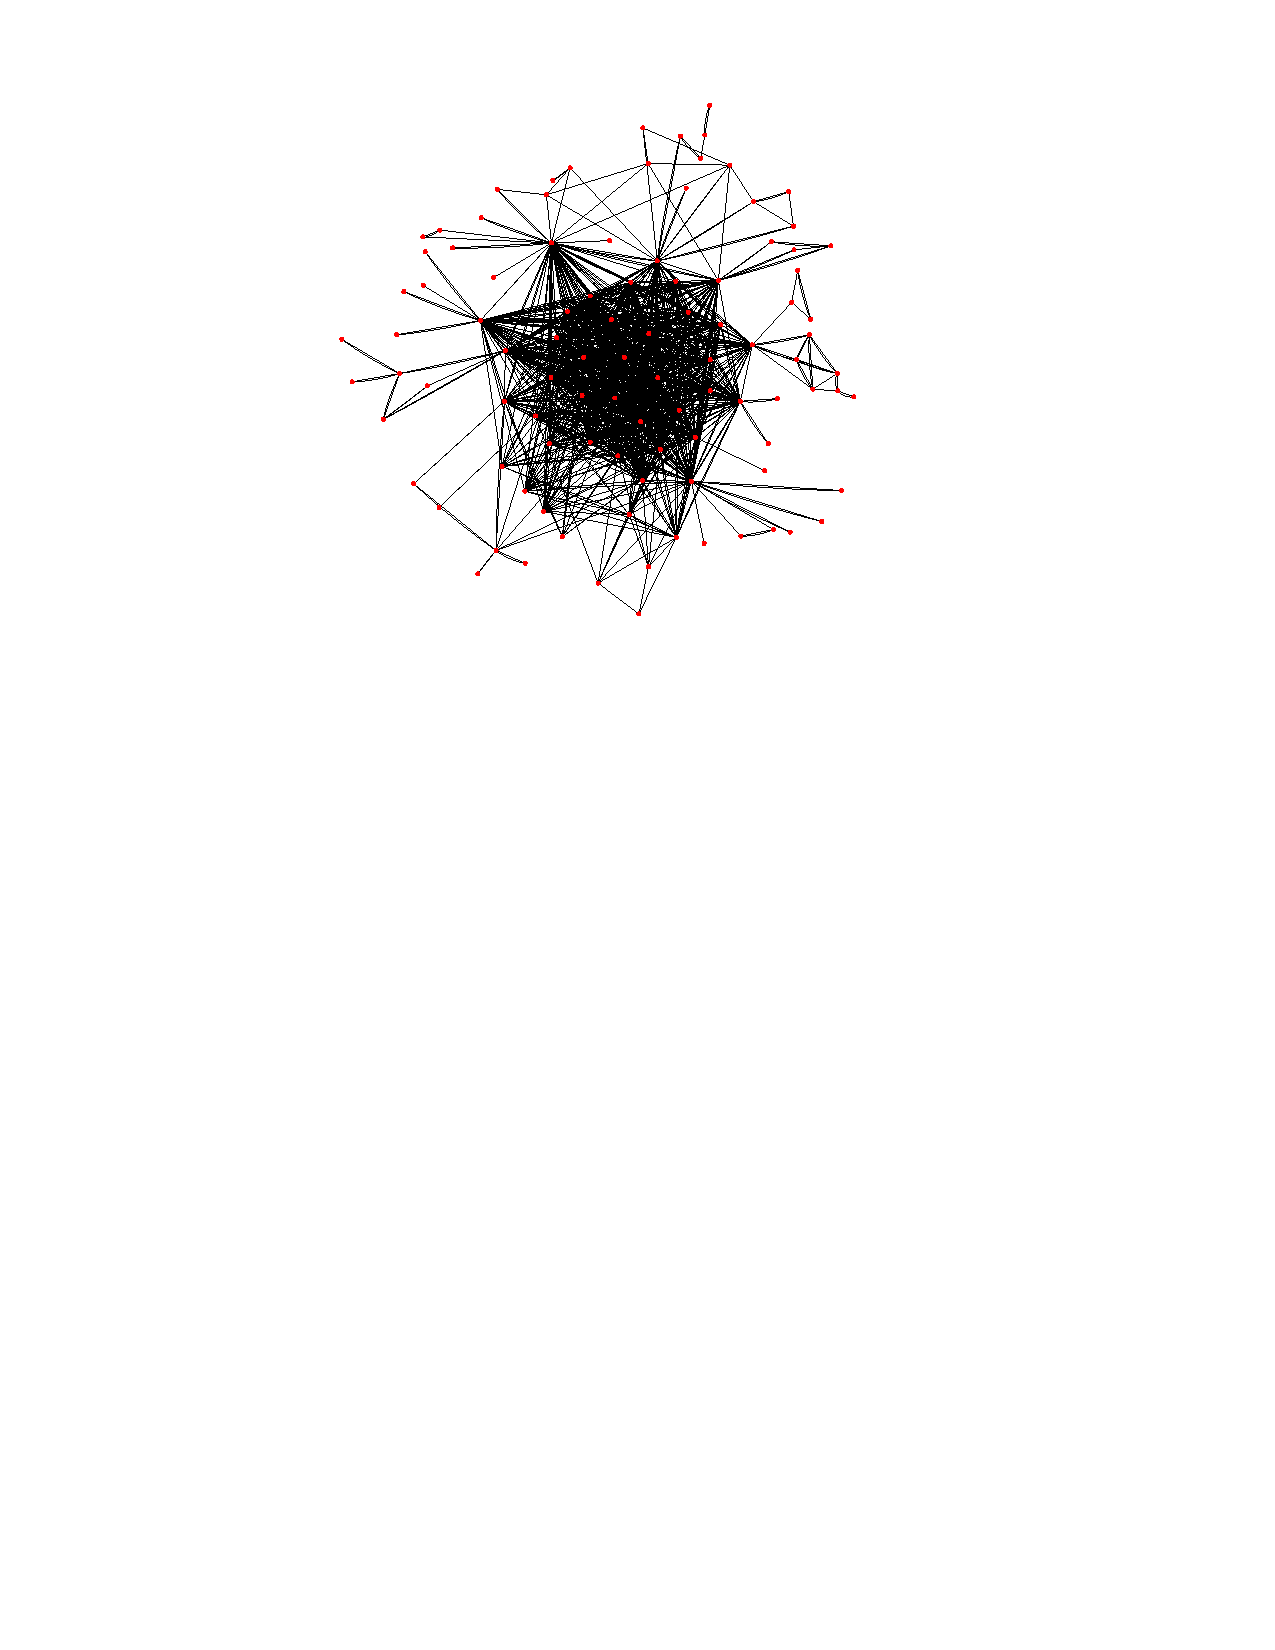
\includegraphics[scale=1.5]{images/subgraph-label-time-fa62cc57cd35e9f90b85435efc407ad5.pdf}
  \caption{Community mit zeitlicher Korrelation der Signaturen
    (Blondel ($l=5$),
    100 Knoten, 72\% der Signaturen innerhalb eines Monats)}
  \label{fig:time-corr-com-normal}
\end{figure}


\begin{figure}[th!]
  \centering
  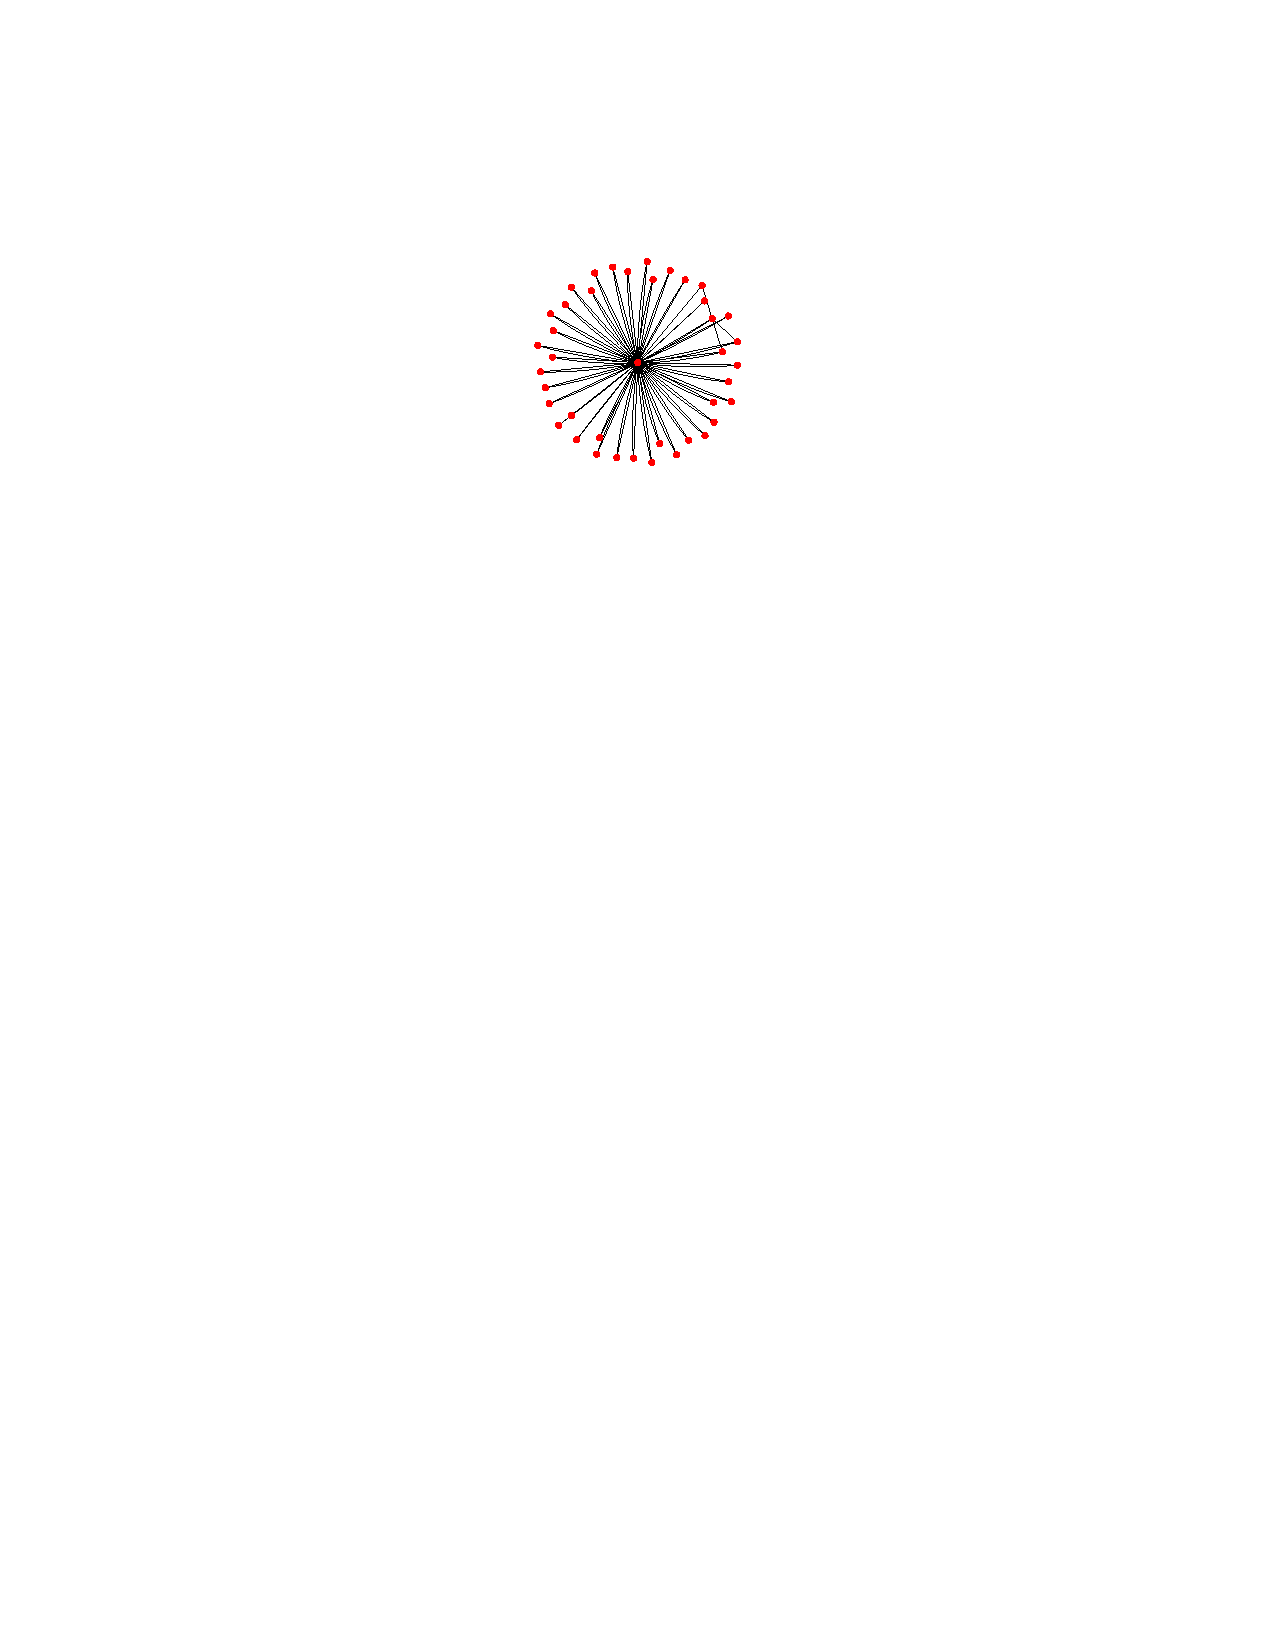
\includegraphics[scale=1.3]{images/label-subgraph-41-star-c222345bc5eb1f9eff80d58a81861974.pdf}
    \caption{Community mit zeitlicher Korrelation der Signaturen
      (Blondel ($l=5$),
      41 Knoten, 84 \% der Signaturen innerhalb eines Monats)}
  \label{fig:time-corr-com-star}
\end{figure}

Es stellt sich die Frage, ob die zeitliche Korrelation der Signaturen
in einer Community ein geeignetes Mittel ist, um Keysigning-Parties zu
erkennen. Neben dem zeitlichen Zusammenhang der Signaturen ist ein
weiteres Merkmal einer Keysigning-Party wie in
Ab. \ref{sec:sozi-komp-des} beschrieben, dass jeder Teilnehmer mit
(fast) jedem anderem Teilnehmer Signaturen austauscht, so dass sich
eine fast vollst\"andige Vermaschung -- fast eine Clique --
ergibt. Eine stichprobenartige Untersuchung in den Communities zeigt,
dass die meisten Communities mit zeitlicher Korrelation zumindest
teilweise dieses Merkmal zeigen. Abbildung
\ref{fig:time-corr-com-normal} zeigt ein Beispiel einer solchen
Community. Etwa die H\"alfte der Knoten ist in einer Fast-Clique
enthalten, deren Knoten mit (fast) allen anderen vernetzt sind. Dieser
innere Teil des Teilgraphen entspricht genau dem Bild, das als
Resultat einer Keysigning-Party erwartet wird. Auch wenn dies auf die
meisten der Communities mit zeitlicher Korrelation zutrifft, gibt es
auch Gegenbeispiele. Abbildung \ref{fig:time-corr-com-star} zeigt eine
Community, die zwar das Kriterium der zeitlichen Korrelation
erf\"ullt, ansonsten aber nichts mit dem erwarteten Bild einer KSP
gemein hat. Allerdings erf\"ullt der Teilgraph trotzdem das Kriterium
der Community, da die Knoten am Rand nur Signaturen zu dem zentralen
Knoten haben und damit die interne Kantendichte deutlich h\"oher ist
als die externe. Um solche Extremf\"alle auszuschliessen, ist als
zus\"atzliches Kriterium f\"ur die Erkennung von KSPs ein hoher
durchschnittlicher Grad der Knoten denkbar.

\begin{figure}[th!]
  \centering
  \subfloat[]{\label{fig:sld-sure-copra1} 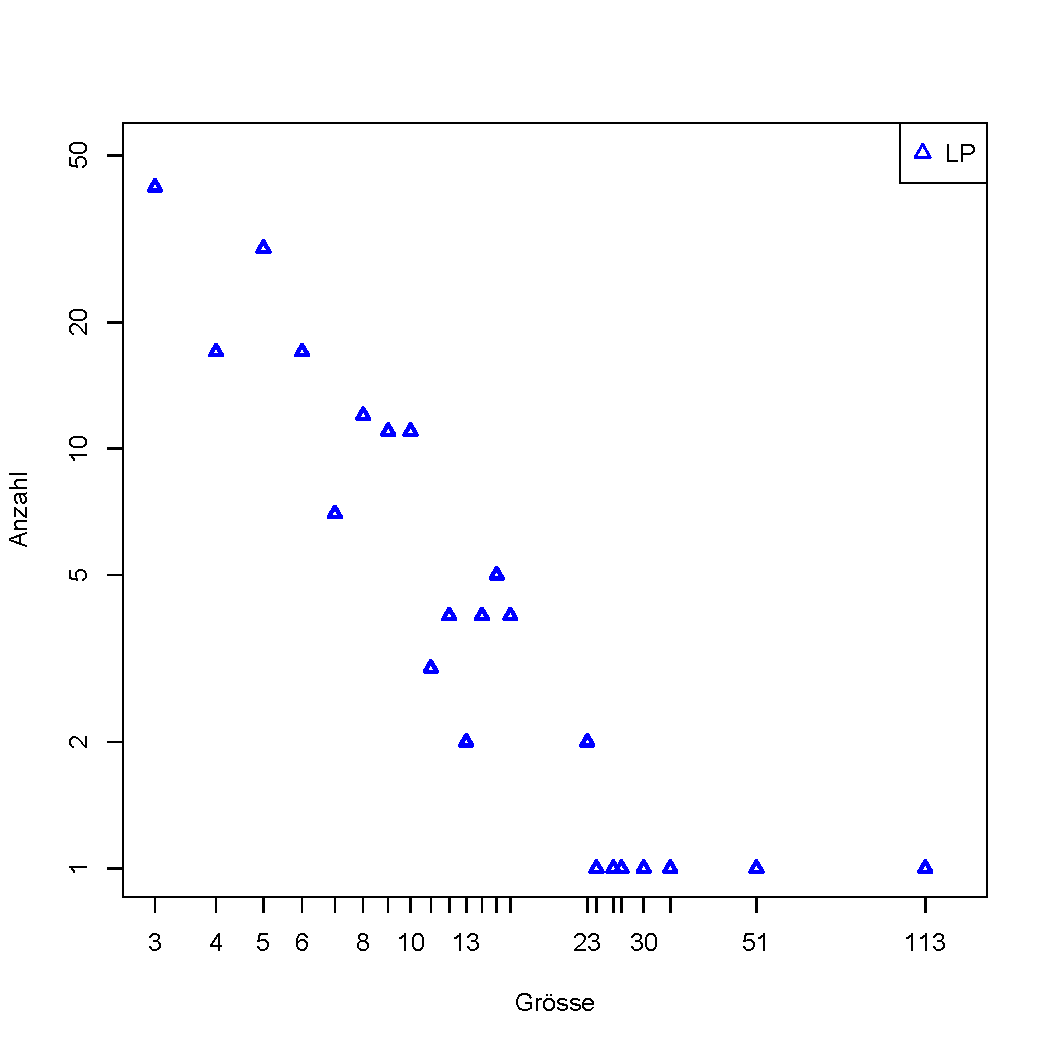
\includegraphics[scale=0.45]{images/sld-sure-ass_copra1.pdf}}
  \subfloat[]{\label{fig:sld-sure-bl2} 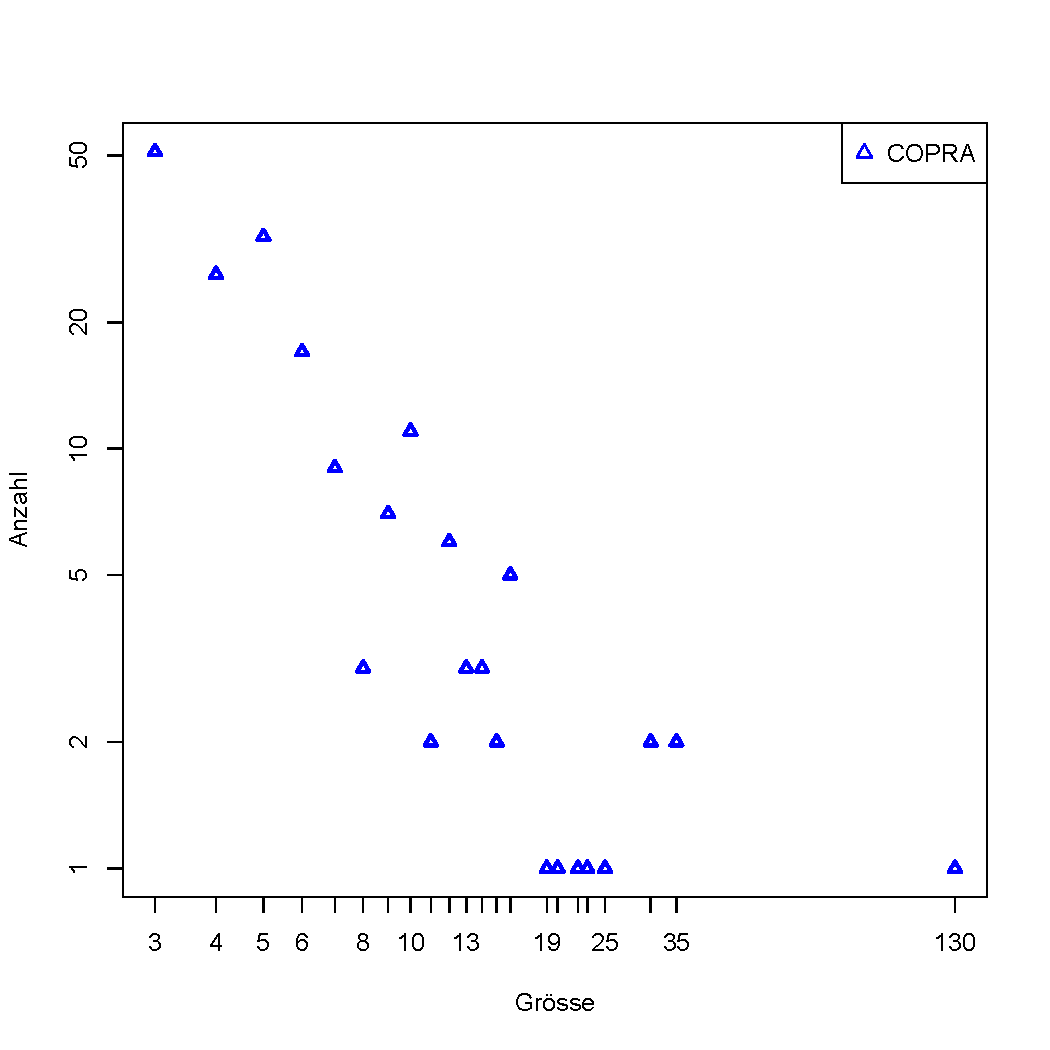
\includegraphics[scale=0.45]{images/sld-sure-ass_copra.pdf}}\\
  \subfloat[]{\label{fig:sld-sure-bl5} 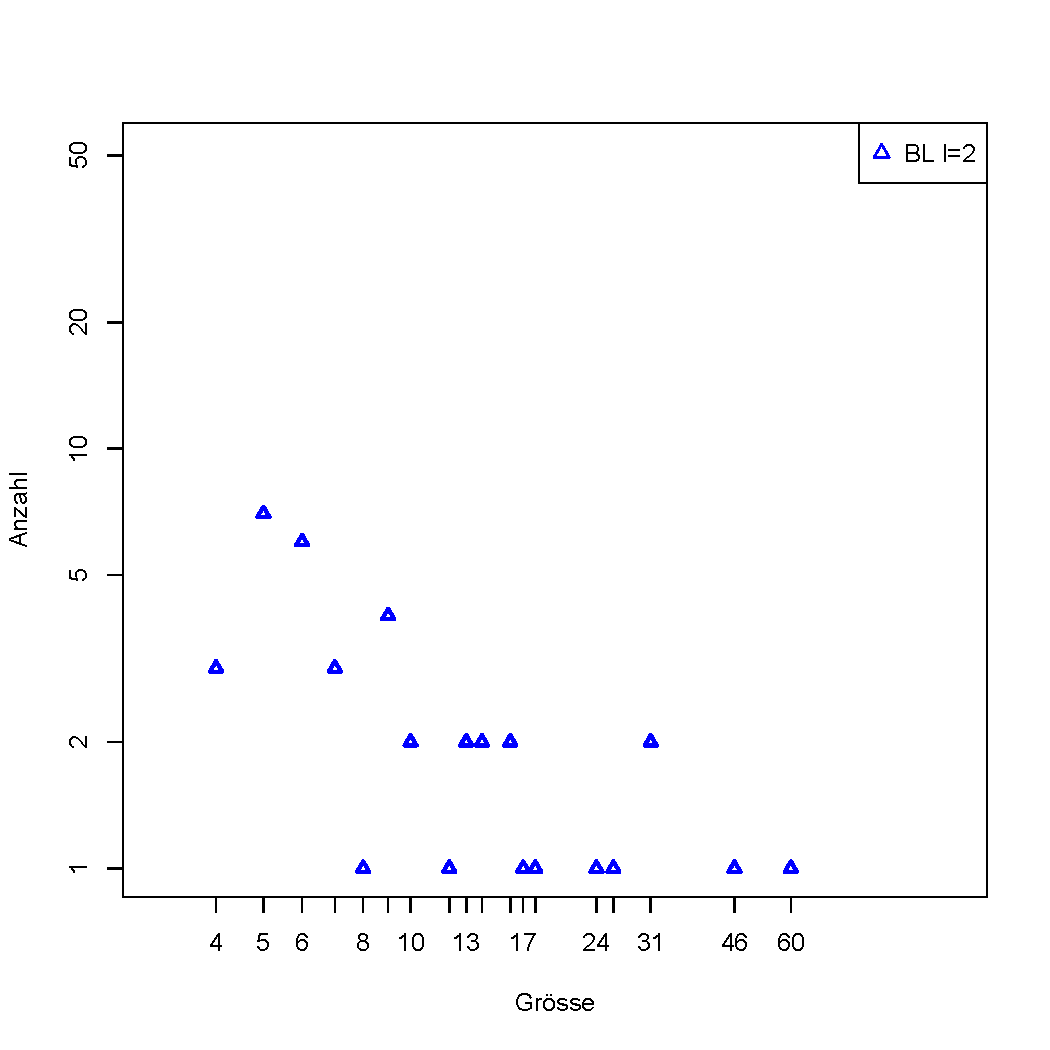
\includegraphics[scale=0.45]{images/sld-sure-ass_bl2.pdf}} 
  \subfloat[]{\label{fig:sld-sure-copra} 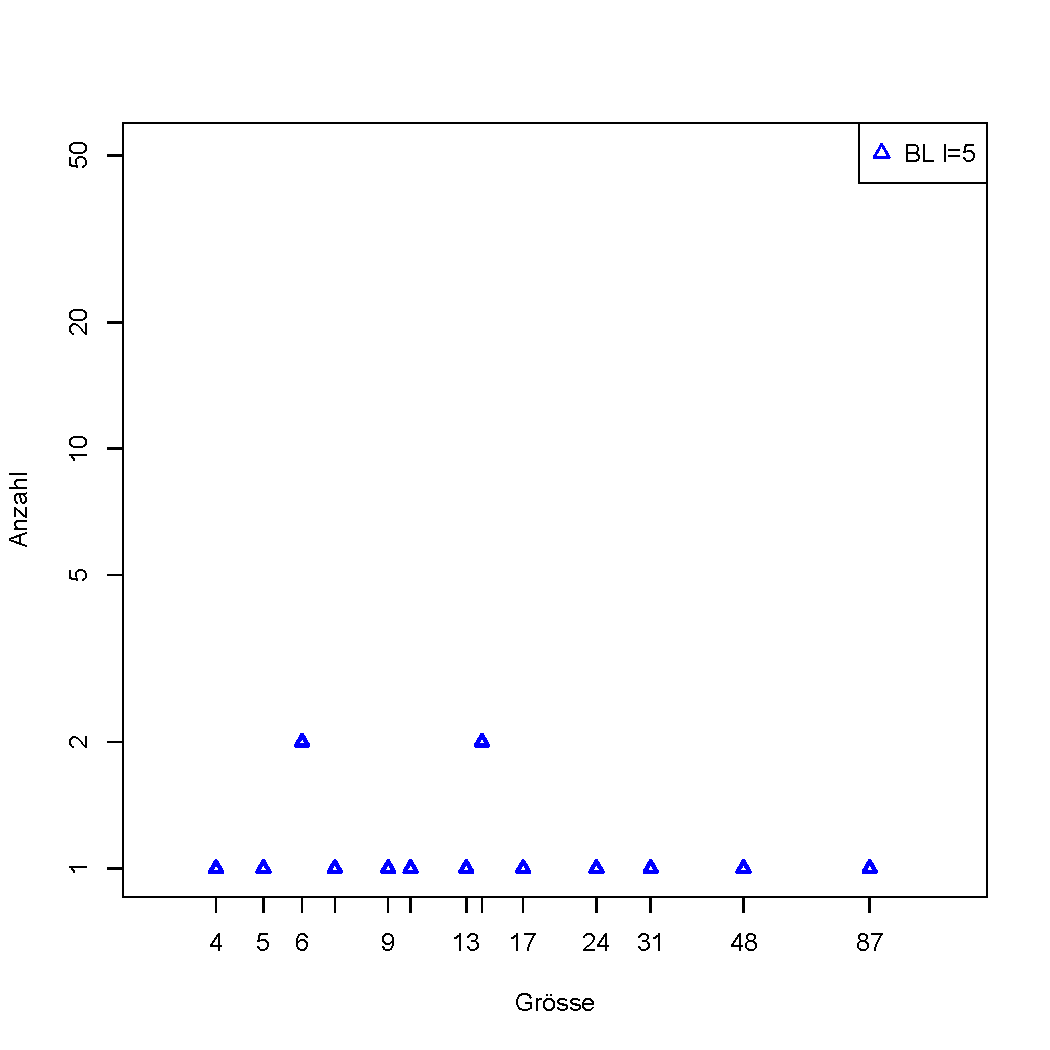
\includegraphics[scale=0.45]{images/sld-sure-ass_bl5.pdf}}
  \caption{Zuweisung von Domains zu SLDs abh\"angig von der Community-Gr\"osse}
  \label{fig:sld-suredist}
\end{figure}

\begin{figure}[th!]
  \centering
  \subfloat[]{\label{fig:sld-maybe-copra1} 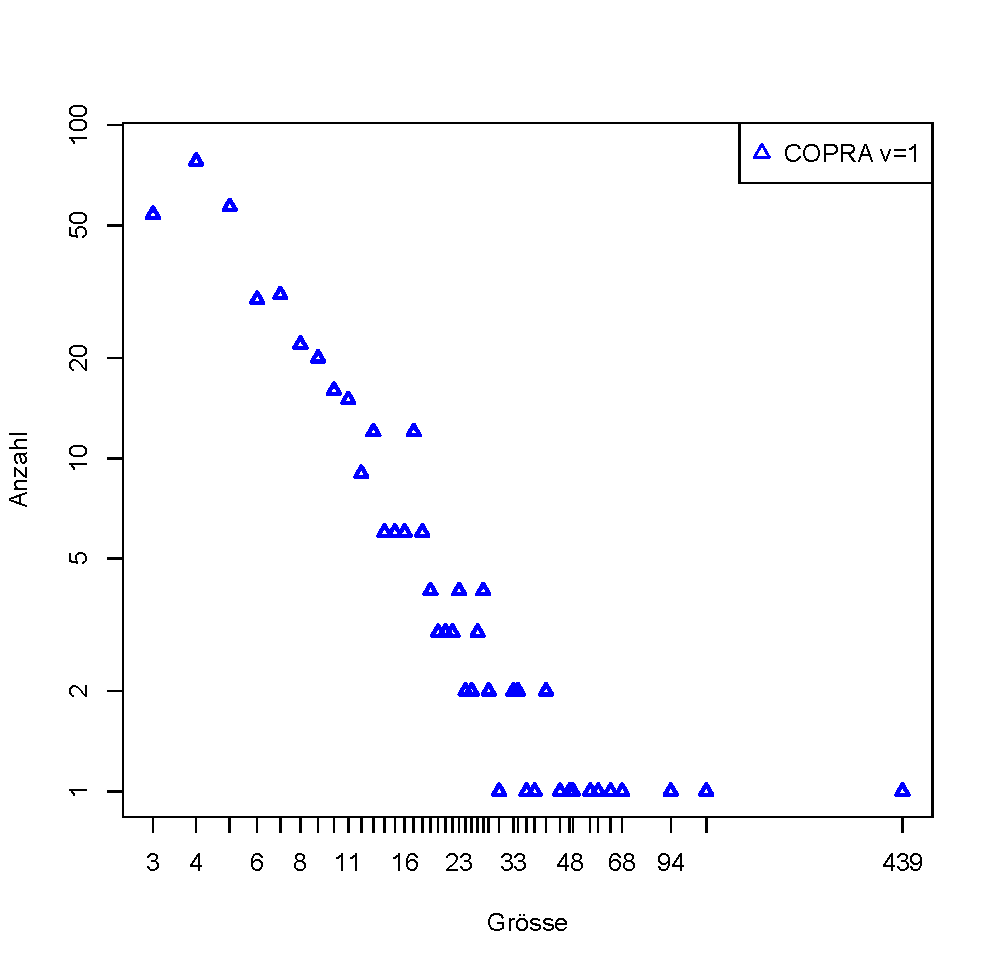
\includegraphics[scale=0.45]{images/sld-maybe-ass_copra1.pdf}}
  \subfloat[]{\label{fig:sld-maybe-bl2} 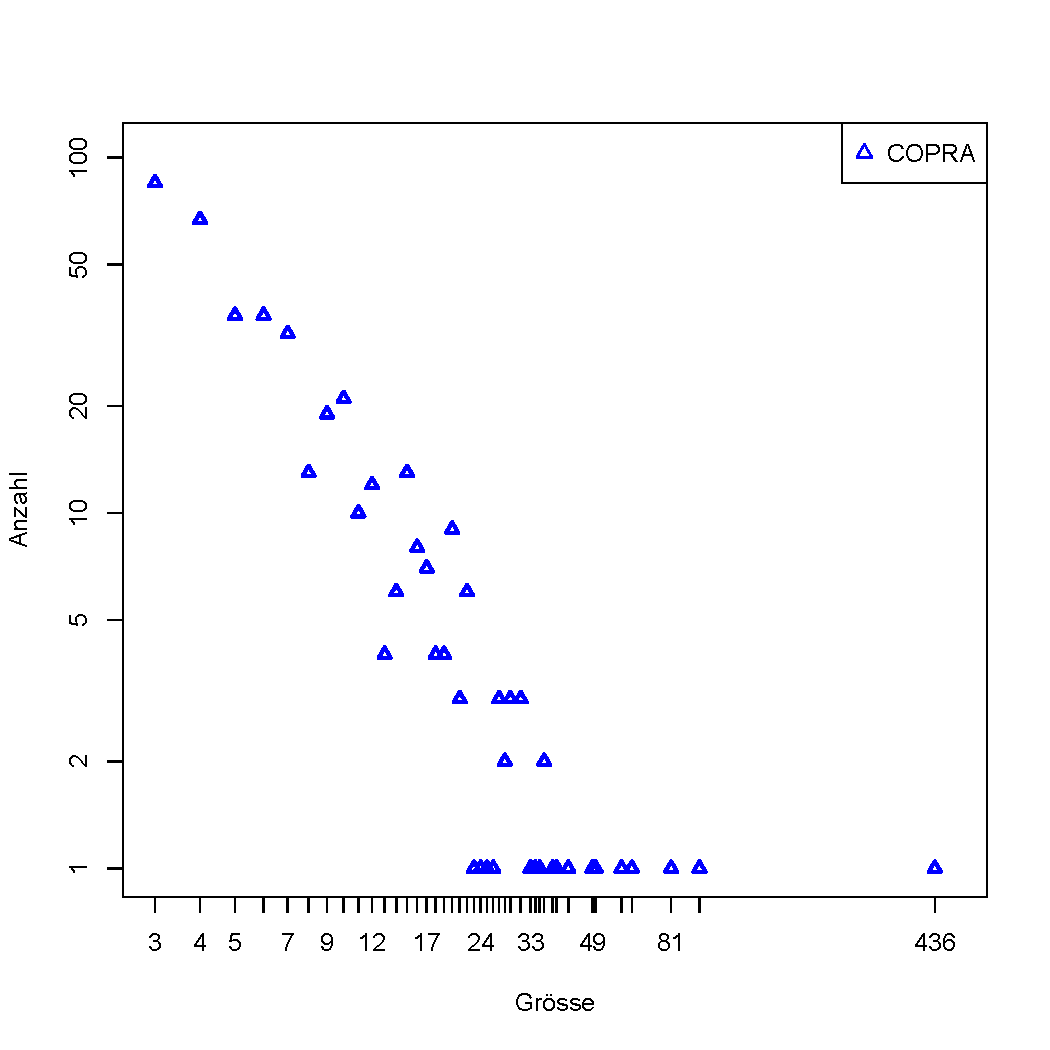
\includegraphics[scale=0.45]{images/sld-maybe-ass_copra.pdf}}\\
  \subfloat[]{\label{fig:sld-maybe-bl5} 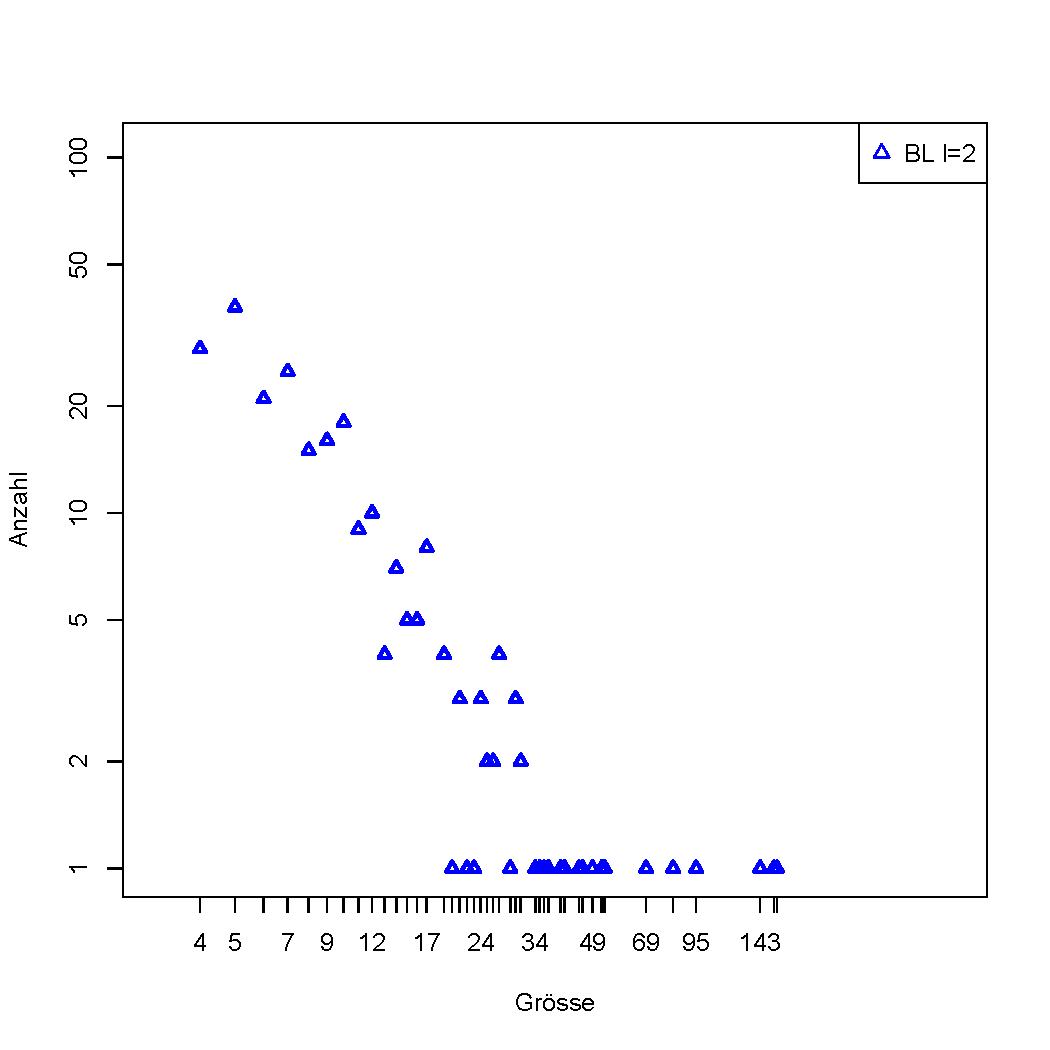
\includegraphics[scale=0.45]{images/sld-maybe-ass_bl2.pdf}} 
  \subfloat[]{\label{fig:sld-maybe-copra} 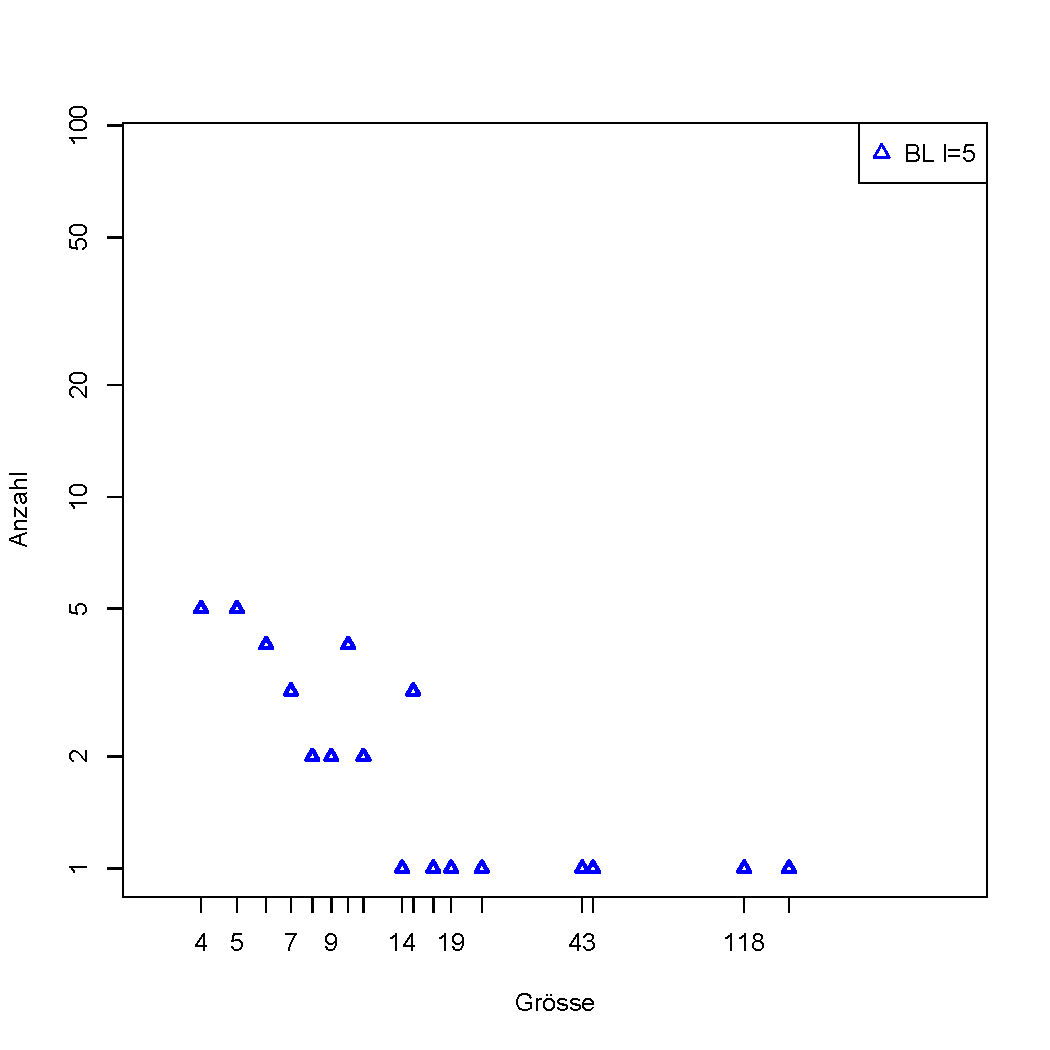
\includegraphics[scale=0.45]{images/sld-maybe-ass_bl5.pdf}}
  \caption{Verteilung der Gr\"osse der von einer SLD dominierten Communities}
  \label{fig:sld-maybedist}
\end{figure}

\begin{figure}[th!]
  \centering
  \subfloat[]{\label{fig:time-corr-copra1} 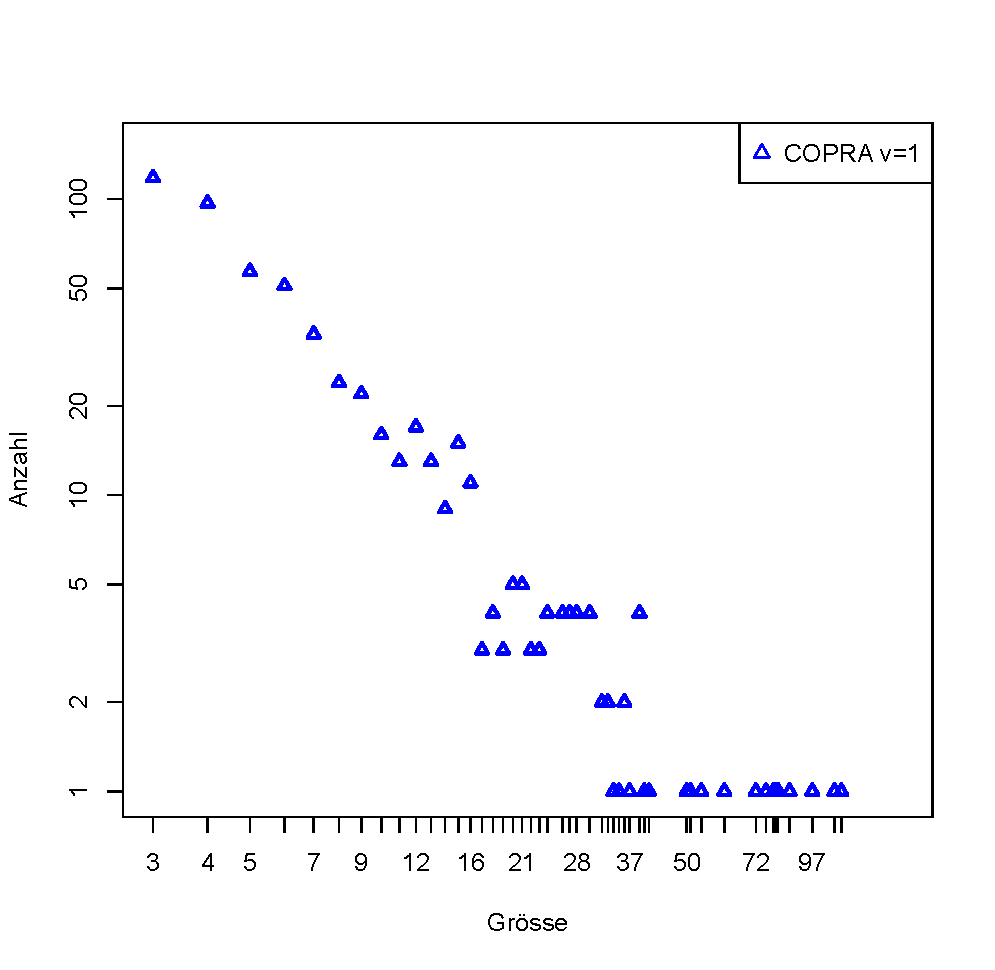
\includegraphics[scale=0.45]{images/time-corr_copra1.pdf}}
  \subfloat[]{\label{fig:time-corr-bl2} 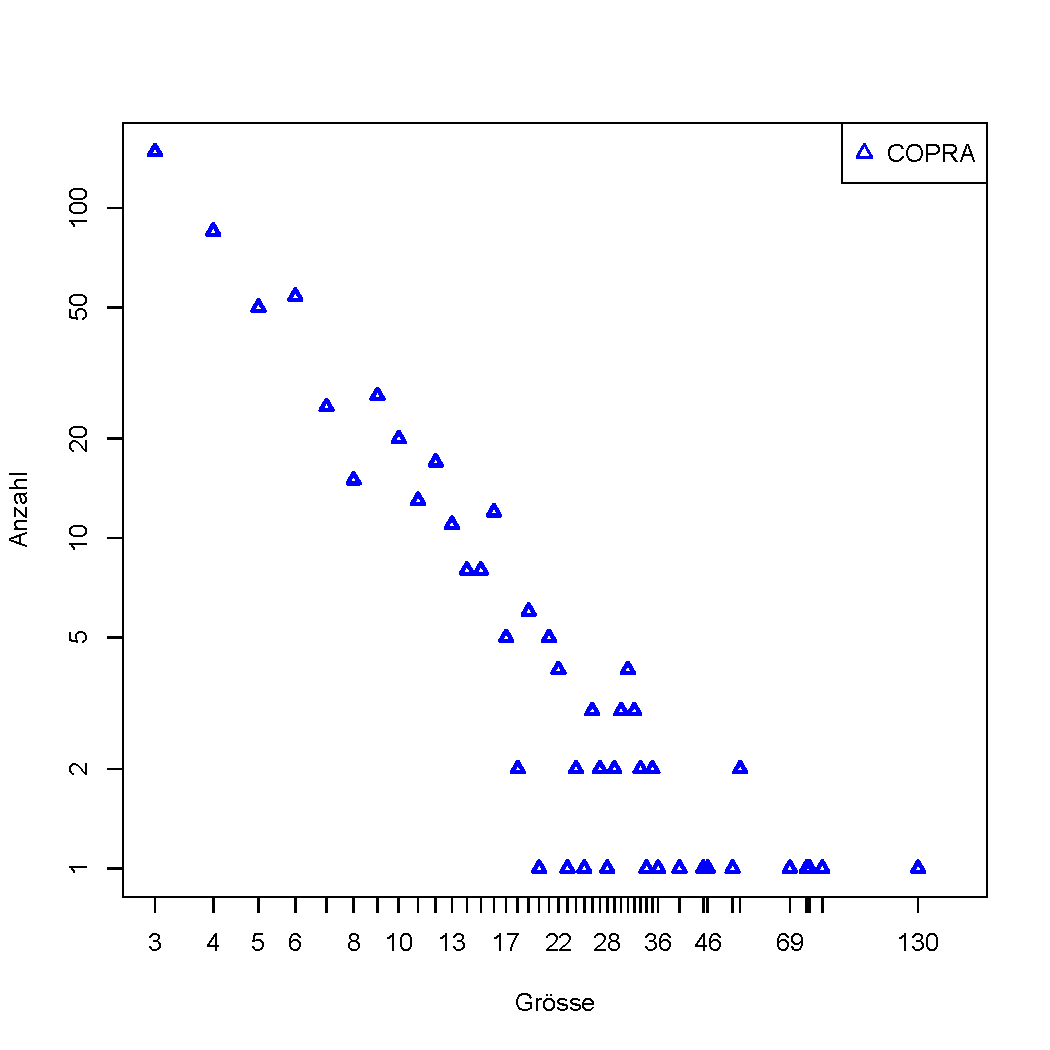
\includegraphics[scale=0.45]{images/time-corr_copra.pdf}}\\
  \subfloat[]{\label{fig:time-corr-bl5} 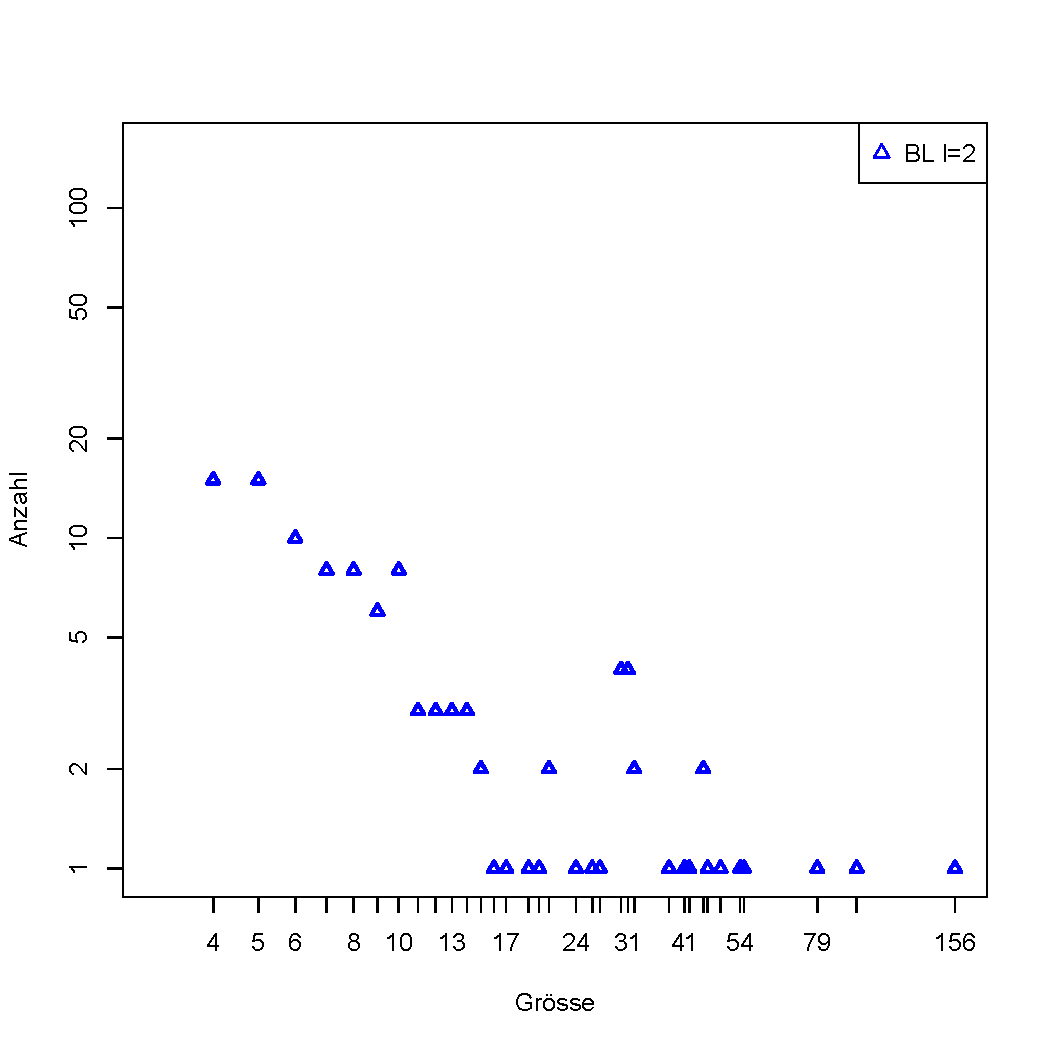
\includegraphics[scale=0.45]{images/time-corr_bl2.pdf}} 
  \subfloat[]{\label{fig:time-corr-copra} 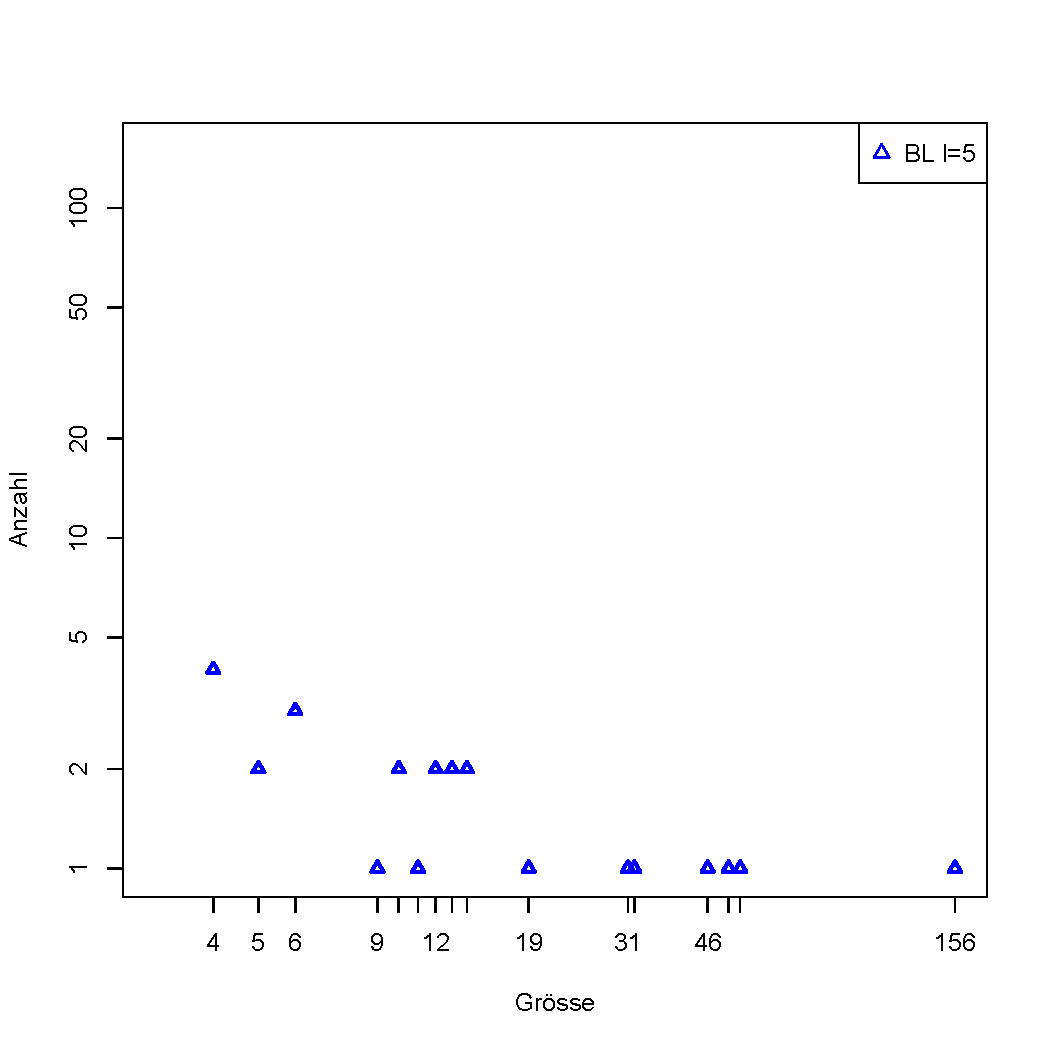
\includegraphics[scale=0.45]{images/time-corr_bl5.pdf}}
  \caption{Verteilung der Gr\"osse von Communities mit zeitlicher
    Korrelation der Signaturen}
  \label{fig:time-corrdist}
\end{figure}

Diese Ergebnisse widerlegen nicht die Annahme, dass die Vernetzung im
Web of Trust im wesentlichen von Keysigning-Parties und den sozialen
Kontakten der Teilnehmer beeinflusst wird und damit unter anderem von
Gruppenzugeh\"origkeit bestimmt wird. Allerdings muss festgehalten
werden, dass die hier verwendeten Methoden nicht geeignet sind, um den
Entstehungsmechanismus entlang dieser Annahme befriedigend zu
erkl\"aren. 

Ein Grund daf\"ur ist sicherlich, dass die Struktur des Web of Trust
nur zu einem bestimmten, festen Zeitpunkt betrachtet wurde. Um die
Entstehungsdynamik zu verstehen, k\"onnte alternativ die Entwicklung
des Netzwerks tats\"achlich \"uber die Zeit nachvollzogen werden. Das
Keyserver-Netzwerk speichert nicht nur den momentanen Zustand des
Netzwerks, sondern implizit auch den Entstehungszeitpunkt jedes
Schl\"ussels und jeder Signatur. Die im Rahmen dieser Arbeit
entwickelte Software speichert diese Zeitstempel in einer Datenbank
und macht so die gesamte Entwicklungsgeschichte des Web of Trust
verf\"ugbar (siehe Abschnitt
\ref{ch:Grundlagen:sec:Design:subsec:eigene-software}). Anhand dieser
Daten k\"onnte nachvollzogen werden, wie und in welcher Form die
Communities tats\"achlich entstehen und sich entwickeln.

Dass nur sehr wenige gr\"ossere Communities mit zeitlicher Korrelation
der Signaturen gefunden wurden, obwohl regelm\"assig gr\"ossere
Keysigning-Parties stattfinden (siehe Abschnitt
\ref{sec:sozi-komp-des}) ist bei n\"ahrerer Betrachtung durchaus
plausibel. Dass eine Keysigning-Party sich in der Struktur markant
abhebt, setzt vorraus, dass ihre Teilnehmer ausser der Teilnahme an
dieser Party keine wesentliche Signaturaktivit\"at starten. W\"urden
sie weiterhin an Signaturaktitiv\"aten teilnehmen, w\"urde die
Struktur der Keysigning-Party mit der Zeit durch Signaturen von und zu
Nicht-Teilnehmern ``verwischt'' werden. Aufgefunden wurden also
vermutlich nur die Keysigning-Parties mit einer Mehrheit von insgesamt
eher inaktiven Teilnehmern. Gleiches kann f\"ur Teilnehmer angenommen
werden, die sich anhand von Gruppenzugeh\"origkeit vernetzen. Auch
hier w\"urde die Struktur mit der Zeit ``unsch\"arfer'' werden, wenn
ihre Mitglieder weiterhin Signierungen vornehmen w\"urden. Es kann
also angenommen werden, dass die kleineren und insbesondere die klar
zuordnenbaren Communities tendenziell Teilnehmer enthalten, die in
Bezug auf die Teilnahme am Web of Trust eher inaktiv sind. Um diese
Vermutung zu best\"atigen oder zu wiederlegen, k\"onnte das
Signaturverhalten der Teilnehmer \"uber die Zeit mit ihrer
Community-Mitgliedschaft verglichen und korreliert werden.

Es scheint unrealistisch, dass die Mitgliedschaft in einer Gruppe --
etwa einer Firma, akademischen Einrichtung oder einem
Open-Source-Projekt -- die sozialen Kontakte einer Person
vollst\"andig charakterisiert. Daneben kann eine Person noch ein
weites Netzwerk an Freunden oder Bekannten haben, die diese
Mitgliedschaft nicht teilen. Trotzdem k\"onnen sich zu ihnen
Signaturen ergeben, die einen wesentlichen Teil der Signaturen dieser
Person ausmachen k\"onnen. Ausserdem ist anzunehmen, dass eine
Vielzahl solcher Gruppen nicht \"uber eine gemeinsame Domain
verf\"ugen, und damit mit den hier vorliegenden Daten schlicht nicht
sichtbar sind. Zwar wurde versucht, der anzunehmenden Komplexit\"at
der Gruppenzugeh\"origkeiten durch \"uberlappende Communities zu
begegnen. Allerdings konnte der verwendete Algorithmus keine
signifikanten \"Uberlappungseigenschaften liefern . Die Frage,
inwiefern sich die einzelnen Communities sozialen Gruppen zuordnen
lassen, konnte also nur unvollst\"andig beantwortet werden.

Es zeigt sich, dass dem Web of Trust kein einzelner, einfacher
Entstehungsmechanismus der hier angenommenen Form zugrundeliegt. Es
kann nur unzureichend beschrieben werden als eine Ansammlung von
einzelnen, einfach entstandenen Bausteinen, als die hier Communities
angenommen wurden. Implizit vorrausgesetzt wird dabei auch, dass diese
zum Beispiel im Fall einer Keysigning-Party nach ihrer Entstehung
keine wesentliche weitere Vernetzungsaktitiv\"at zeigen. Zwar trifft
dies f\"ur einen Teil der Communities -- gerade die, die eine
zeitliche Korrelation der Signaturen zeigen oder einer
Second-Level-Domain zugeordnet werden k\"onnen -- durchaus zu. F\"ur
einen erheblichen Anteil der Teilnehmer -- beispielsweise die
Mitglieder der sehr grossen Community aus der COPRA-Berechnung --
scheint die Vernetzung jedoch so vielf\"altig zu sein, dass solche
einfachen Mechanismen nicht mehr sichtbar sind und ``in der Masse
verschwinden''. Bei der COPRA-Zerlegung ist es etwa naheliegend, dass
die sehr grosse zentrale Community die Mehrzahl der aktiveren
Teilnehmer enth\"alt. Hier ergibt sich eine \"Ahnlichkeit zur Struktur
der Zusammenhangskomponenten, bei denen die gr\"osste alle aktiven
einigermassen aktiven Teilnehmer zu enthalten scheint (siehe Abschnitt
\ref{sec:zusammenhangskomponenten-inhaltlich}).

Diese Punkte k\"onnen anhand des Beispiels von Debian illustriert
werden: Das Debian-Projekt als tats\"achliche Community, in der
PGP und das Web of Trust eine besonders wichtige Rolle spielen (siehe
Abschnitt \ref{sec:sozi-komp-des}) findet sich in den Zerlegungen
nicht als eigene abgregrenzte Einheit wieder. Statt dessen finden sich
sehr grosse Communities, in denen Debian-Entwickler einen signifikaten
Anteil der Schl\"ussel stellen. Im Fall der COPRA-Zerlegung ist dies
die bereits erw\"ahnte Community mit ca. 21000 Mitgliedern. Von diesen
verf\"ugen 1247 \"uber eine E-Mail-Adresse in der Domain debian.org
und sind damit offensichtlich Mitglieder des Debian-Projekts. Daneben
finden sich Mitglieder des Debian-Projekts in einer Vielzahl von
kleineren Communities aller Gr\"ossen. Die Mitgliedschaft im
Debian-Projekt scheint hier also f\"ur die Vernetzung keine so
wesentliche Rolle zu spielen, dass sie die Struktur dieser real
existierenden Community im Web of Trust wiederspiegelt. Selbst wenn viele
Debian-Entwickler mit vielen anderen Projektmitgliedern vernetzt sind,
so verf\"ugen sie offensichtlich \"uber gen\"ugend andere Kontakte,
so dass diese Struktur nicht mehr auffindbar ist.

\subsection{Inhaltliche Analyse der Zusammenhangskomponenten}
\label{sec:zusammenhangskomponenten-inhaltlich}

Starke Zusammenhangskomponenten k\"onnen als ein Extremfall von
Communities betrachtet werden, also Mengen von Knoten, die intern
st\"arker vernetzt sind als extern. 

\begin{itemize}
\item strange Komponenten mit unklarer Funktion: kaos.org,
  ethereal.com, ...

\item Bei den kleineren (<20): Viele Komponenten, die mehrere
  Schluessel einer Person enthalten oder nur aus einer Person
  bestehen
\item Komponente aus einer einzelnen Firma, keine weitere
  Vernetzung. Schl\"ussel werden vermutlich nur intern benutzt. Stellt
  aber einen effektiven Ersatz f\"ur eine CA zur Absicherung der
  internen Kommunikation dar (Serco, ponl).
\end{itemize}

Ergebniss: bei den kleineren Komponenten handelt es sich entweder um
komplett geschlossene ``Communities'', deren Teilnehmer von vornherein
nur an der Community selbst interessiert sind oder um Gruppen, die so
inaktiv sind, dass es f\"ur eine weitere Vernetzung nicht gereicht
hat.



%%% Local Variables: 
%%% mode: latex
%%% TeX-master: "diplarb"
%%% End: 

